\documentclass[10pt, aspectratio=43]{beamer}
% \usetheme{Warsaw}
\usetheme{Szeged}
\usecolortheme{beaver}
% \usecolortheme{beaver}
\usepackage{hyperref}
% \usepackage{enumitem}

\setbeamertemplate{page number in head/foot}[totalframenumber]
\setbeamertemplate{caption}[numbered]
\setbeamertemplate{navigation symbols}{}

\usepackage[T1,T2A]{fontenc}
\usepackage[utf8]{inputenc}
\usepackage[english,russian]{babel}

\usepackage{graphicx}%Вставка картинок правильная
\usepackage[caption=false]{subfig}
\usepackage[export]{adjustbox}
\usepackage{float}%"Плавающие" картинки
\usepackage{wrapfig}%Обтекание фигур (таблиц, картинок и прочего)
\usepackage[figurename=Рисунок]{caption}

\PassOptionsToPackage{demo}{graphicx}
\makeatletter
\newcommand\titlegraphicii[1]{\def\inserttitlegraphicii{#1}}
\titlegraphicii{}
\setbeamertemplate{title page}
{
\begin{centering}
    \begin{beamercolorbox}[sep=8pt,center]{institute}
        \usebeamerfont{institute}\insertinstitute
    \end{beamercolorbox}

    \vfill

    \begin{beamercolorbox}[sep=8pt,center]{title}
        \usebeamerfont{title}\inserttitle\par%
        \ifx\insertsubtitle\@empty%
        \else%
        \vskip0.25em%
        {\usebeamerfont{subtitle}\usebeamercolor[fg]{subtitle}\insertsubtitle\par}%
        \fi%
    \end{beamercolorbox}%

% \end{centering}

    \vskip1em\par
    \begin{beamercolorbox}[sep=4pt,right]{author}
    \footnotesize
    \textbf{Автор:} \\ \insertauthor \\
    \textbf{Научный руководитель:} \\
        старший преподаватель,\\
        к.ф.-м.н., Сыч Томаш Сергеевич \\
    \textbf{Рецензент:} \\
        ведущий специалист,\\
        д.ф.-м.н., Колесников Илья Евгеньевич\\
    \end{beamercolorbox}

% \begin{centering}
\vfill
    \vskip1em\par
    \begin{beamercolorbox}[sep=4pt,center]{date}
        \usebeamerfont{date}\insertdate
    \end{beamercolorbox} \vskip0.5em
\end{centering}

}
\makeatother

\title[]{Дизайн сенсоров на основе кластеров золота, стабилизированных аминокислотной матрицей}
\author{Шишкевич Даниил}
\institute[]{Кафедра молекулярной биофизики и физики полимеров \\ Физический факультет \\ Санкт-Петербургский государственный университет}
\date{Санкт-Петербург, 2026 г.}

\begin{document}


\begin{frame}[plain]
    \maketitle
\end{frame}

\begin{frame}{Введение}
    \begin{columns}

    \column{0.5\textwidth}
        \begin{block}{Металлический нанокластер}
            \scriptsize Металлическим кластером называется объект, состоящий из нескольких (от единиц до десятков) атомов металла, который обладает молекулярной электронно-энергетической структурой, а также может поглощать и испускать фотоны.
        \end{block}

        \begin{figure}
            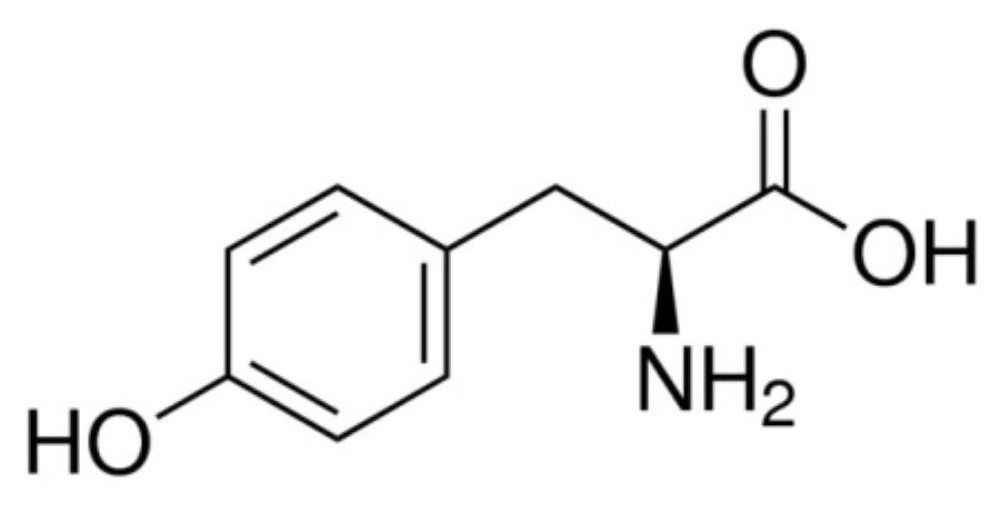
\includegraphics[width=1\linewidth]{attachments/t3754-50g.jpg}
            \caption{\centering \footnotesize Структурная формула L-тирозина}
        \end{figure}

    \column{0.5\textwidth}
        \begin{figure}
            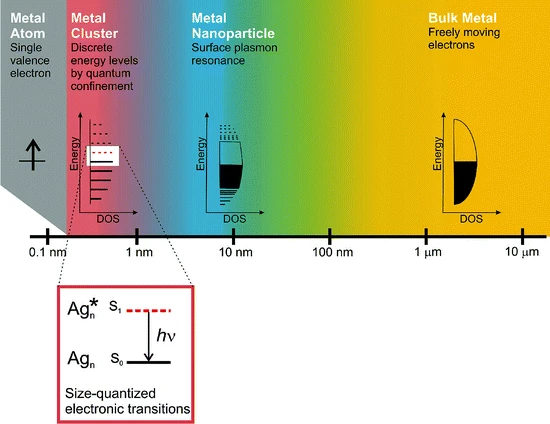
\includegraphics[width=1\linewidth]{attachments/978-3-642-04701-5_10_Fig1_HTML.png}
            \caption{\centering Сравнительная схема электронно-энергетических свойств металла в зависимости от его размера [1]}
        \end{figure}

    \end{columns}
    \Tiny \textcolor{gray}{[1] Díez I., Ras R. H. A. Few-Atom Silver Clusters as Fluorescent Reporters // Advanced Fluorescence Reporters in Chemistry and Biology II, 2010. — С. 307—332.}
\end{frame}

\begin{frame}{Цели и задачи}
    % \centering
    \begin{beamercolorbox}[sep=8pt,left]{Цель}
    \textbf{Цель:}
        Создать простую, биосовместимую и эффективную сенсорную систему на ионы металлов.
    \end{beamercolorbox}

    \begin{beamercolorbox}[sep=8pt,left]{Цель}
    \textbf{Задачи:}
    \begin{enumerate}
        \item синтезировать золотой нанокластер, стабилизированный тирозином;
        \item определить фотофизические характеристики металлического нанокластера;
        \item оценить чувствительность металлического нанокластера;
        \item предложить возможный механизм взаимодействия металлического нанокластера с аналитами.
    \end{enumerate}
    \end{beamercolorbox}

\end{frame}

\begin{frame}{Материалы и методы}
    \setlength{\leftmargini}{0pt}
    % \setlength{\labelsep}{0pt}
    \begin{columns}
        \column[t]{0.65\linewidth}
            \textbf{Методы исследования:}
            \begin{itemize}
                \item[-] Спектроскопия поглощения;
                \item[-] Спектроскопия люминесценции;
                \item[-] Времякоррелированный счёт единичных фотонов.
            \end{itemize}
            \begin{figure}
                \centering
                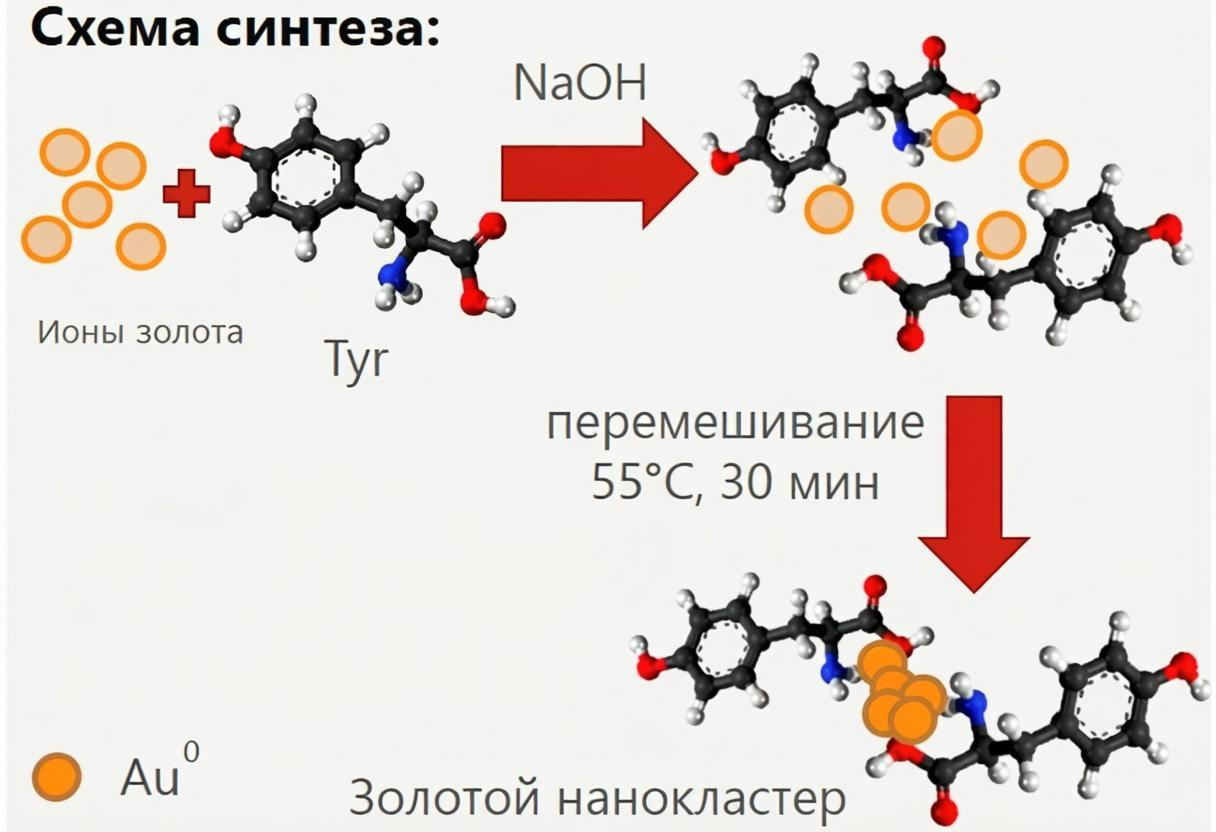
\includegraphics[width=.95\linewidth]{attachments/synthesis-sceme.jpeg}
            \end{figure}

        \column[t]{0.35\linewidth}
        \textbf{Материалы:}
            \begin{itemize}
                \item[-] Соли металлов: \\
                \footnotesize
                \(\mathrm{MnCl_{2}\!\cdot\!4\,\mathrm{H_{2}O}}\),\\
                \(\mathrm{FeSO_{4}\!\cdot\!7\,\mathrm{H_{2}O}}\),\\
                \(\mathrm{FeCl_{3}\!\cdot\!6\,\mathrm{H_{2}O}}\),\\
                \(\mathrm{Cd\!\left(\mathrm{NO}_{3}\right)_{2}\!\cdot\!4\,\mathrm{H_{2}O}}\),\\
                \(\mathrm{CoCl_{2}\!\cdot\!6\,\mathrm{H_{2}O}}\),\\
                \(\mathrm{Cr\!\left(\mathrm{NO}_{3}\right)_{3}\!\cdot\!9\,\mathrm{H_{2}O}}\),
                \(\mathrm{CuSO_{4}\!\cdot\!5\,\mathrm{H_{2}O}}\),
                \(\mathrm{Pb\!\left(\mathrm{NO}_{3}\right)_{2}}\),
                \(\mathrm{AlCl_{3}}\),
                \(\mathrm{NaCl}\),
                \(\mathrm{ZnCl_{2}}\),\\
                \(\mathrm{KCl}\),
                \(\mathrm{NiCl_{2}}\),
                \(\mathrm{CsCl}\)
                \item[-] Гидроксид натрия $\text{NaOH}$;
                \item[-] Вода высокой степени очистки (SQ, $\text{R} > 18.2\text{M}\Omega$)
                \item[-] Тетрахлораурат водорода $\text{H}[\text{AuCl}_4]$
            \end{itemize}
            \vfill
    \end{columns}

\end{frame}

\begin{frame}{Синтез золотого нанокластера}
    \begin{columns}
        \column{0.5\linewidth}
            \textbf{Протокол синтеза:}
            \begin{itemize}
                \item \footnotesize Раствор тирозина ($\text{V}=1~\text{мл};$\\ $\text{C}=0.1~\text{мг}\cdot\text{мл}^{-1};\ \text{pH}=12$)
                \item \footnotesize $\text{HAuCl}_4$ ($\text{V}=2.75~\text{мкл};$\ $\text{C}=0.1~\text{моль}\cdot\text{л}^{-1}$)
                \item \footnotesize 30-минутная инкубация при $55^\circ \text{C}$
            \end{itemize}

            \textbf{Характеризация кластера:}
            \begin{itemize}
                \item \footnotesize Максимум поглощения: 290~нм
                \item \footnotesize Поглощение золотых наночастиц: 520~нм
                \item \footnotesize Максимум возбуждения: 315~нм
                \item \footnotesize Максимум испускания: 405~нм
                \item \footnotesize Время жизни люминесценции: 4.02~нс
                \item \footnotesize Квантовый выход: 3~\%.
            \end{itemize}
        \column{0.6\linewidth}
        \begin{figure}
            \centering
            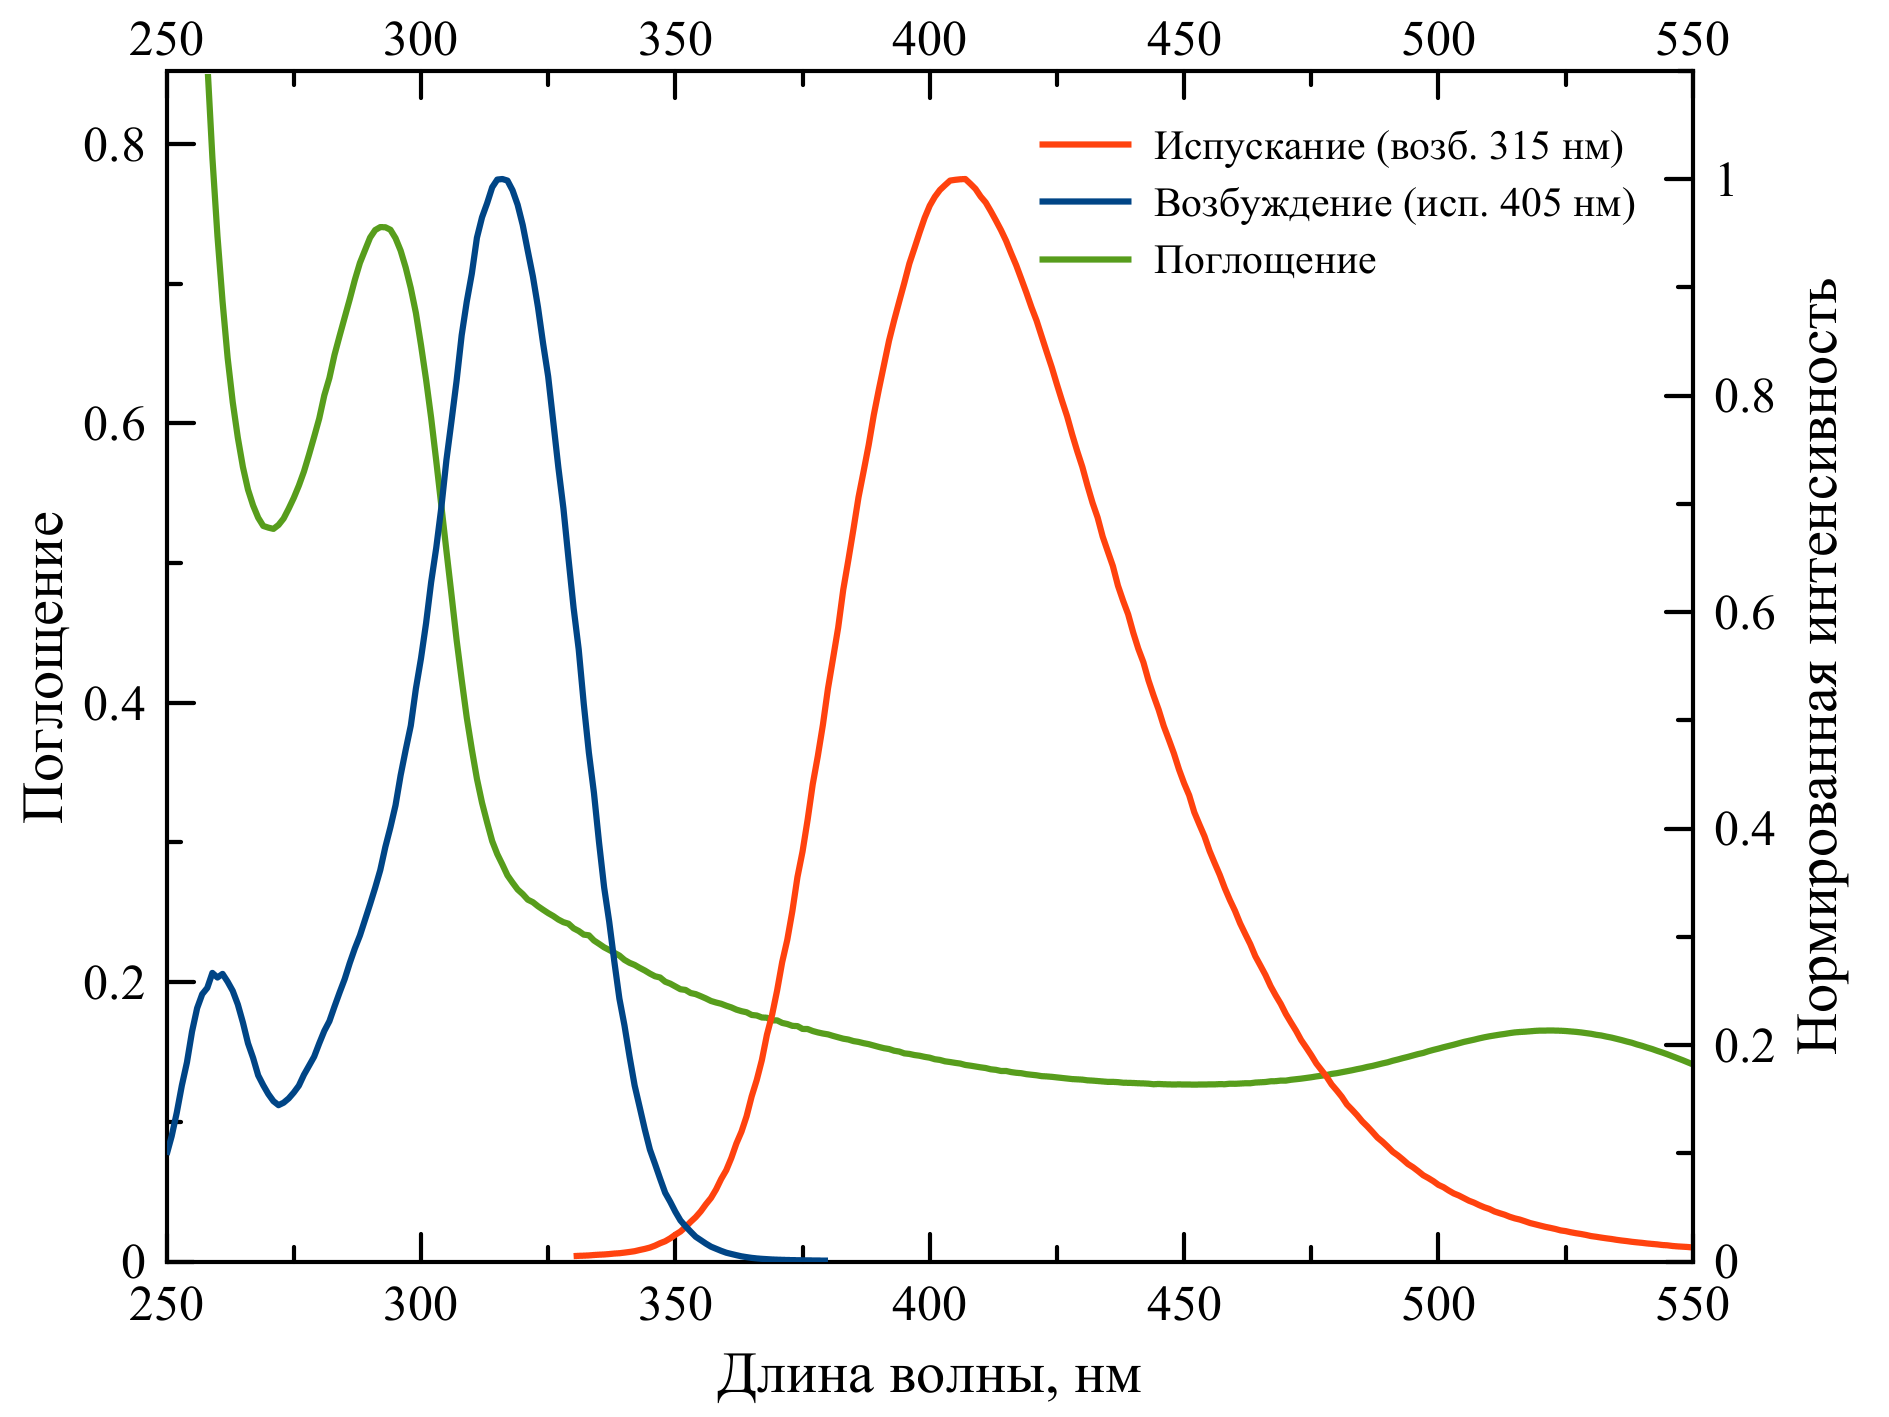
\includegraphics[width=1\linewidth]{attachments/ex_em_abs.png}
            \caption{\centering \footnotesize Спектры поглощения, возбуждения и испускания золотых нанокластеров стабилизированных тирозином.}
        \end{figure}
    \end{columns}
\end{frame}

\begin{frame}{Характеризация золотого нанокластера}
    \begin{columns}[T]
        \column{0.55\linewidth}
            \begin{figure}
            \centering
            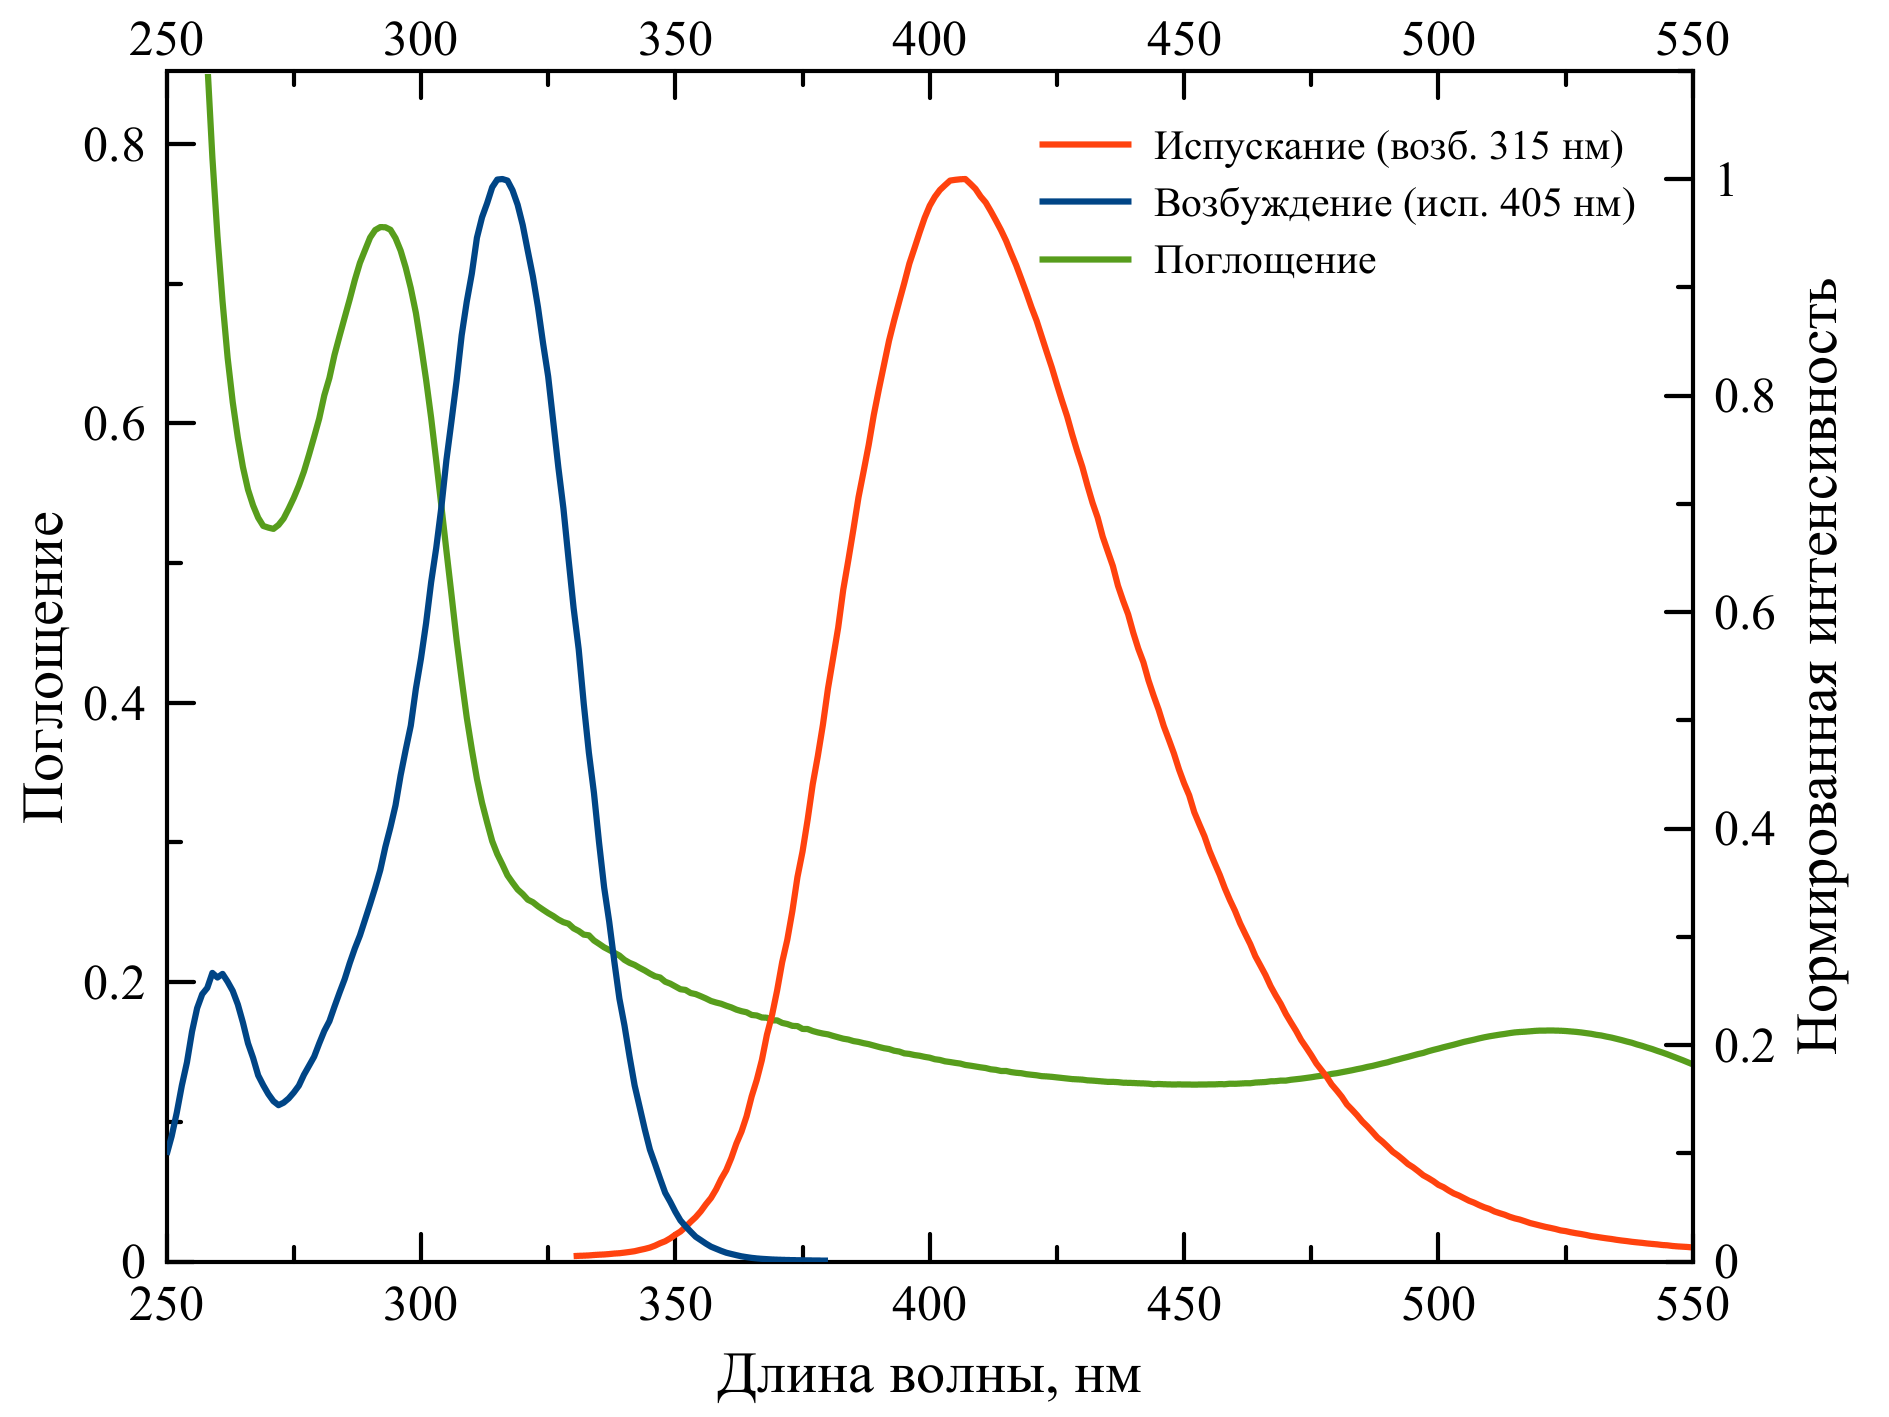
\includegraphics[width=1\linewidth]{attachments/ex_em_abs.png}
            \caption{\centering \footnotesize Спектры поглощения, возбуждения и испускания золотых нанокластеров стабилизированных тирозином.}
        \end{figure}
        \hfill
        \column{0.6\linewidth}
        \begin{figure}
            \centering
            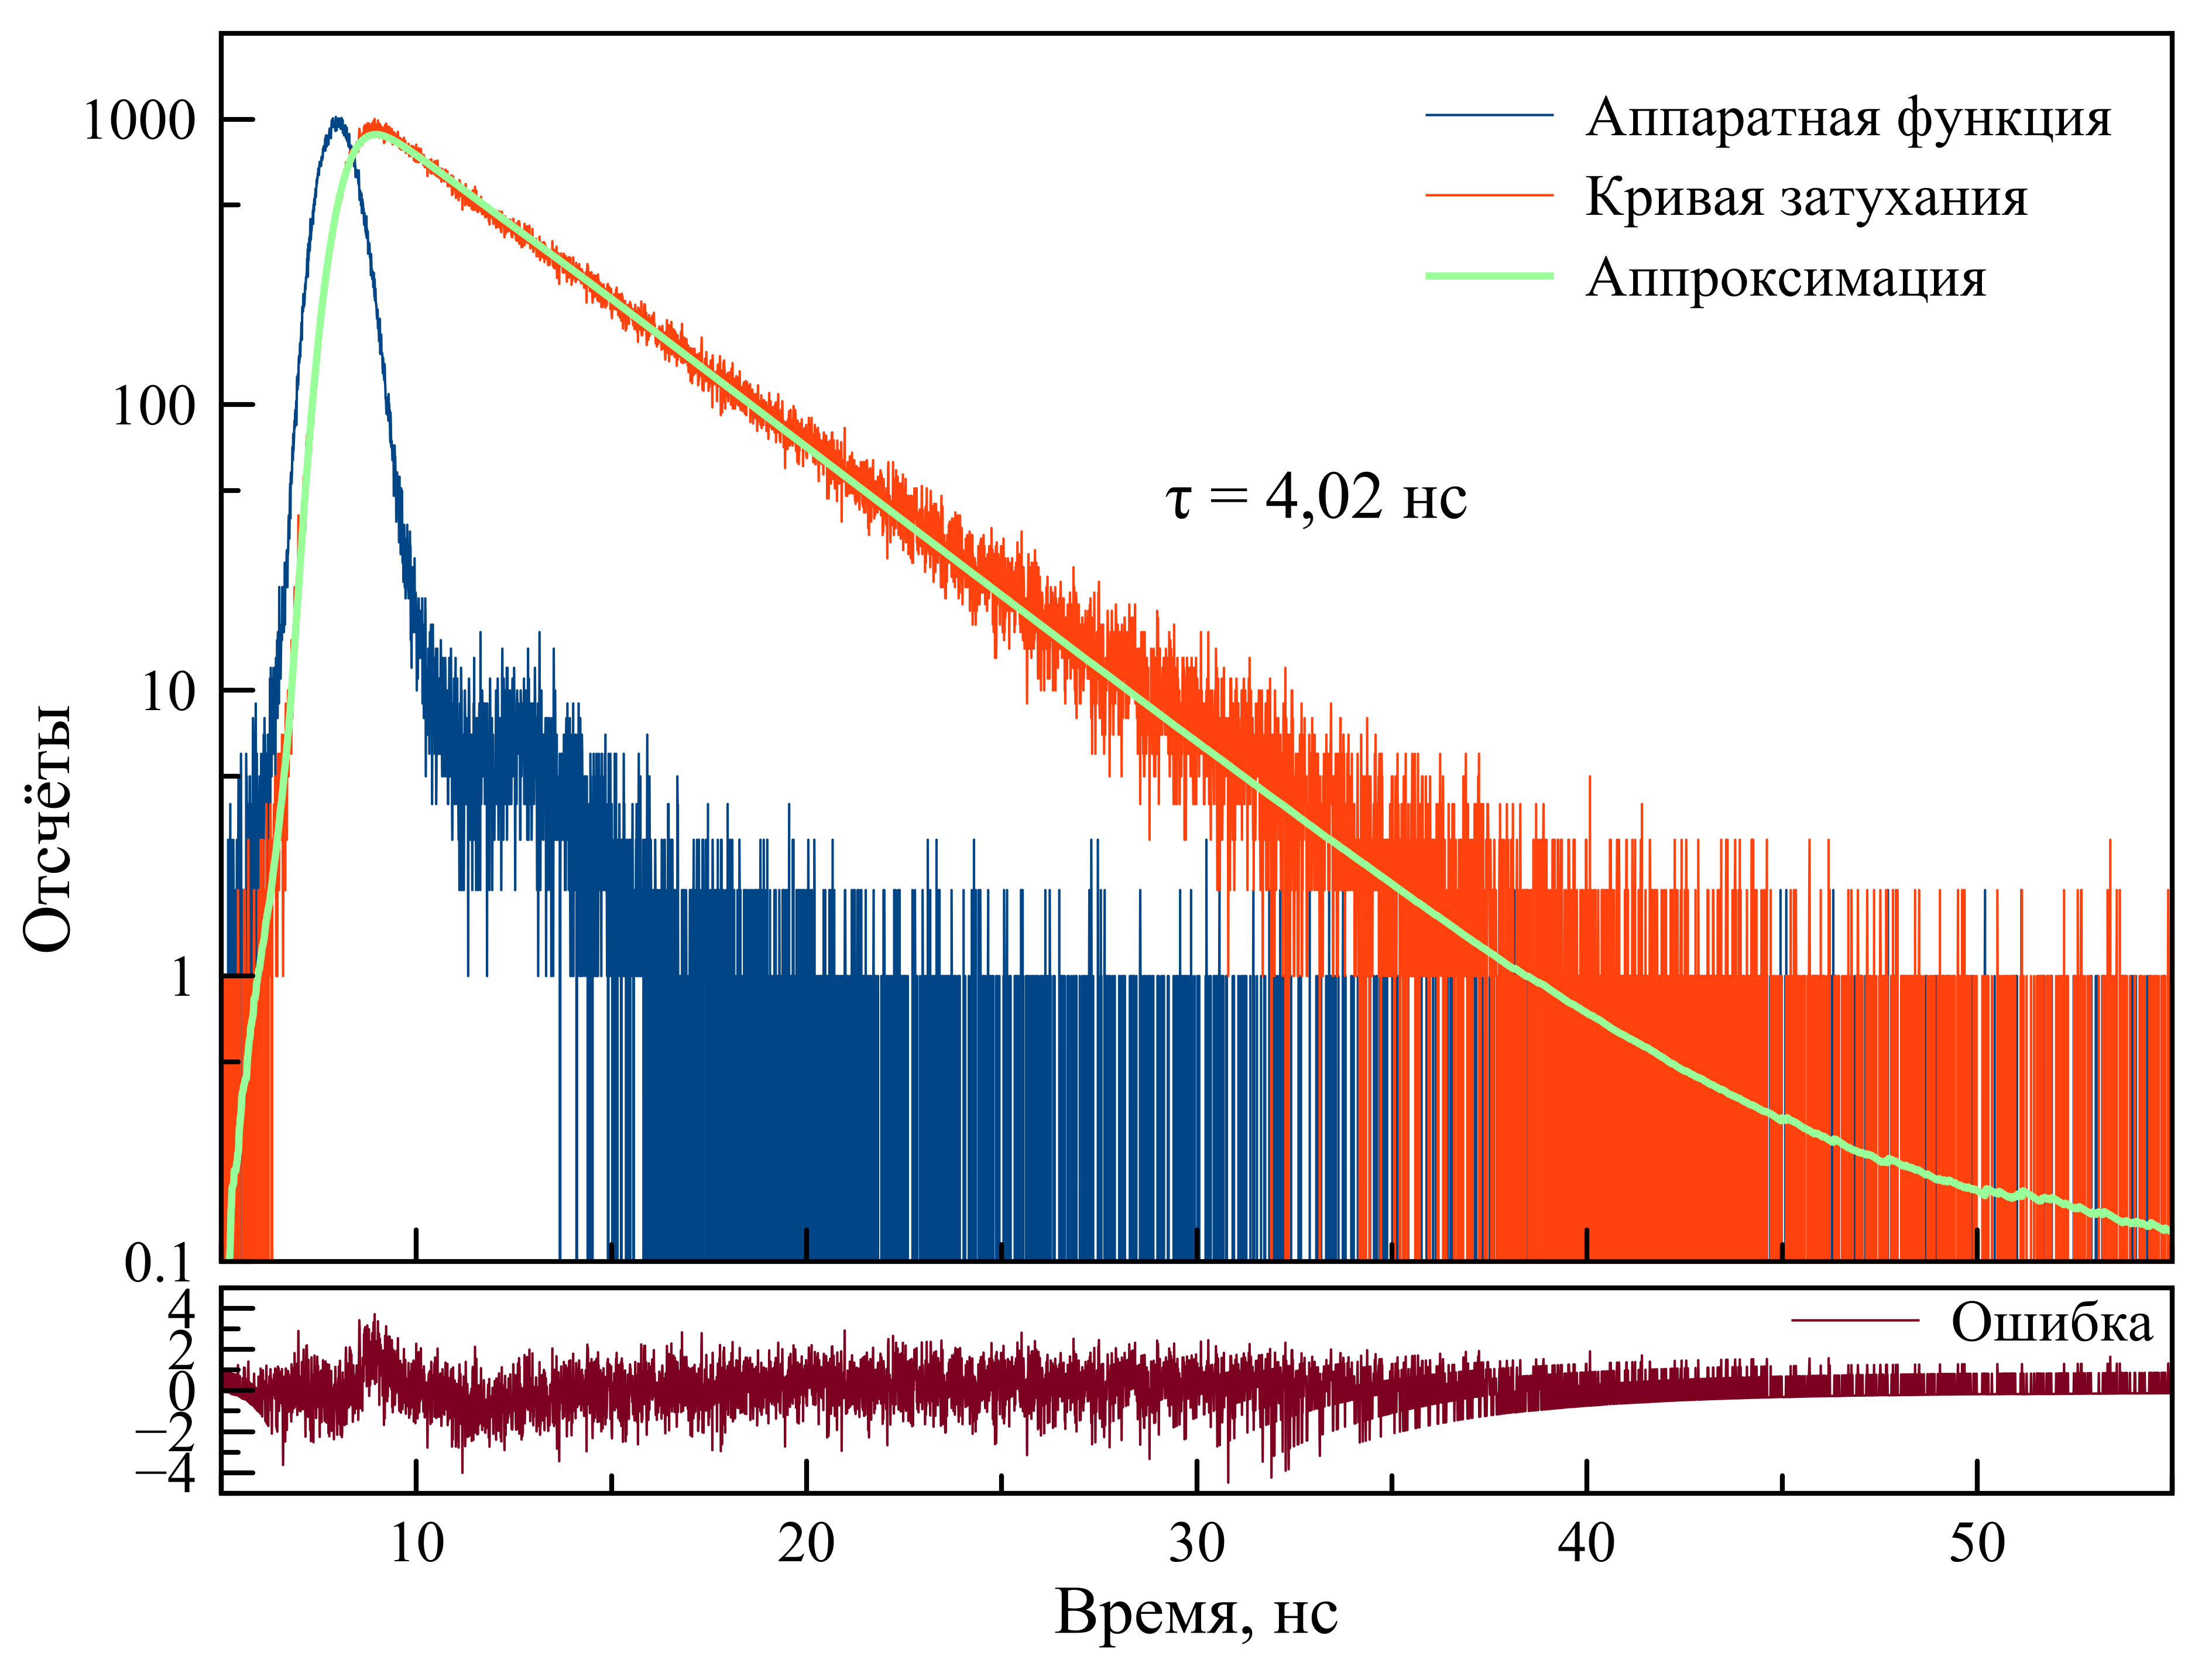
\includegraphics[width=1\linewidth]{attachments/au lifetime.png}
            \caption{\centering \footnotesize Кривая затухания люминесценции золотого нанокластера.}
        \end{figure}
    \end{columns}
\end{frame}

\begin{frame}{Сенсорное применение нанокластера}
\small Различные аналиты (соли металлов) были добавлены к синтезированному нанокластеру и инкубировались при комнатной температуре в течение 15~минут.
    \vfill
    \begin{figure}
        \centering
        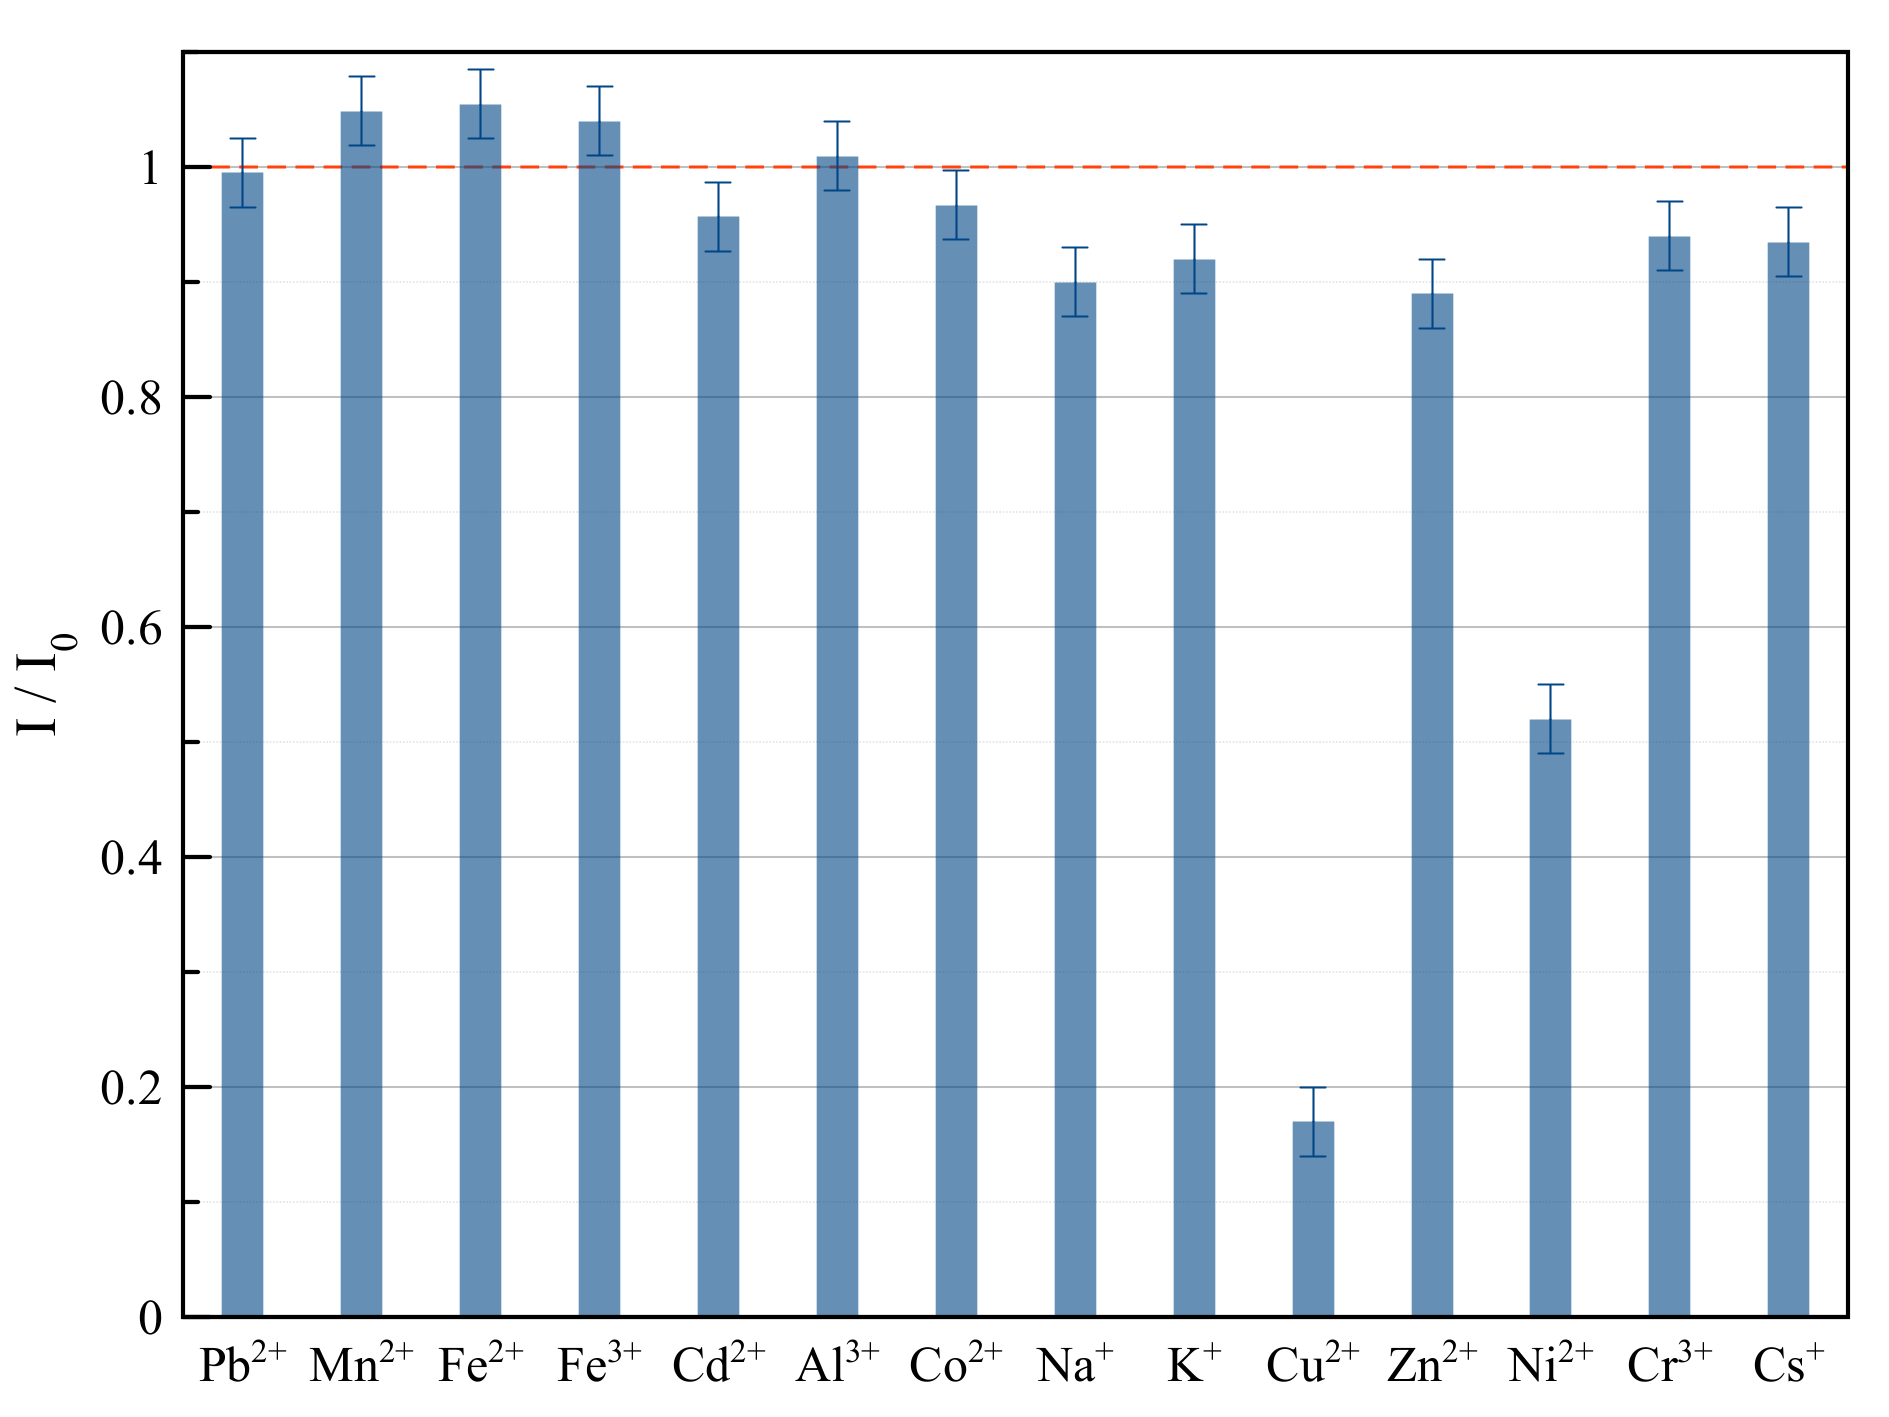
\includegraphics[width=0.60\linewidth]{attachments/metals-compare_opacity.png}
        \caption{\centering Относительная интенсивность люминесценции кластера в присутствии ионов металлов в концентрации 100~$\text{мкмоль}/\text{л}$}
    \end{figure}
\end{frame}

\begin{frame}{Взаимодействие с аналитами: никель}
    \centering
    \begin{columns}[T]
        \column{0.55\linewidth}
        \begin{figure}
            \centering
            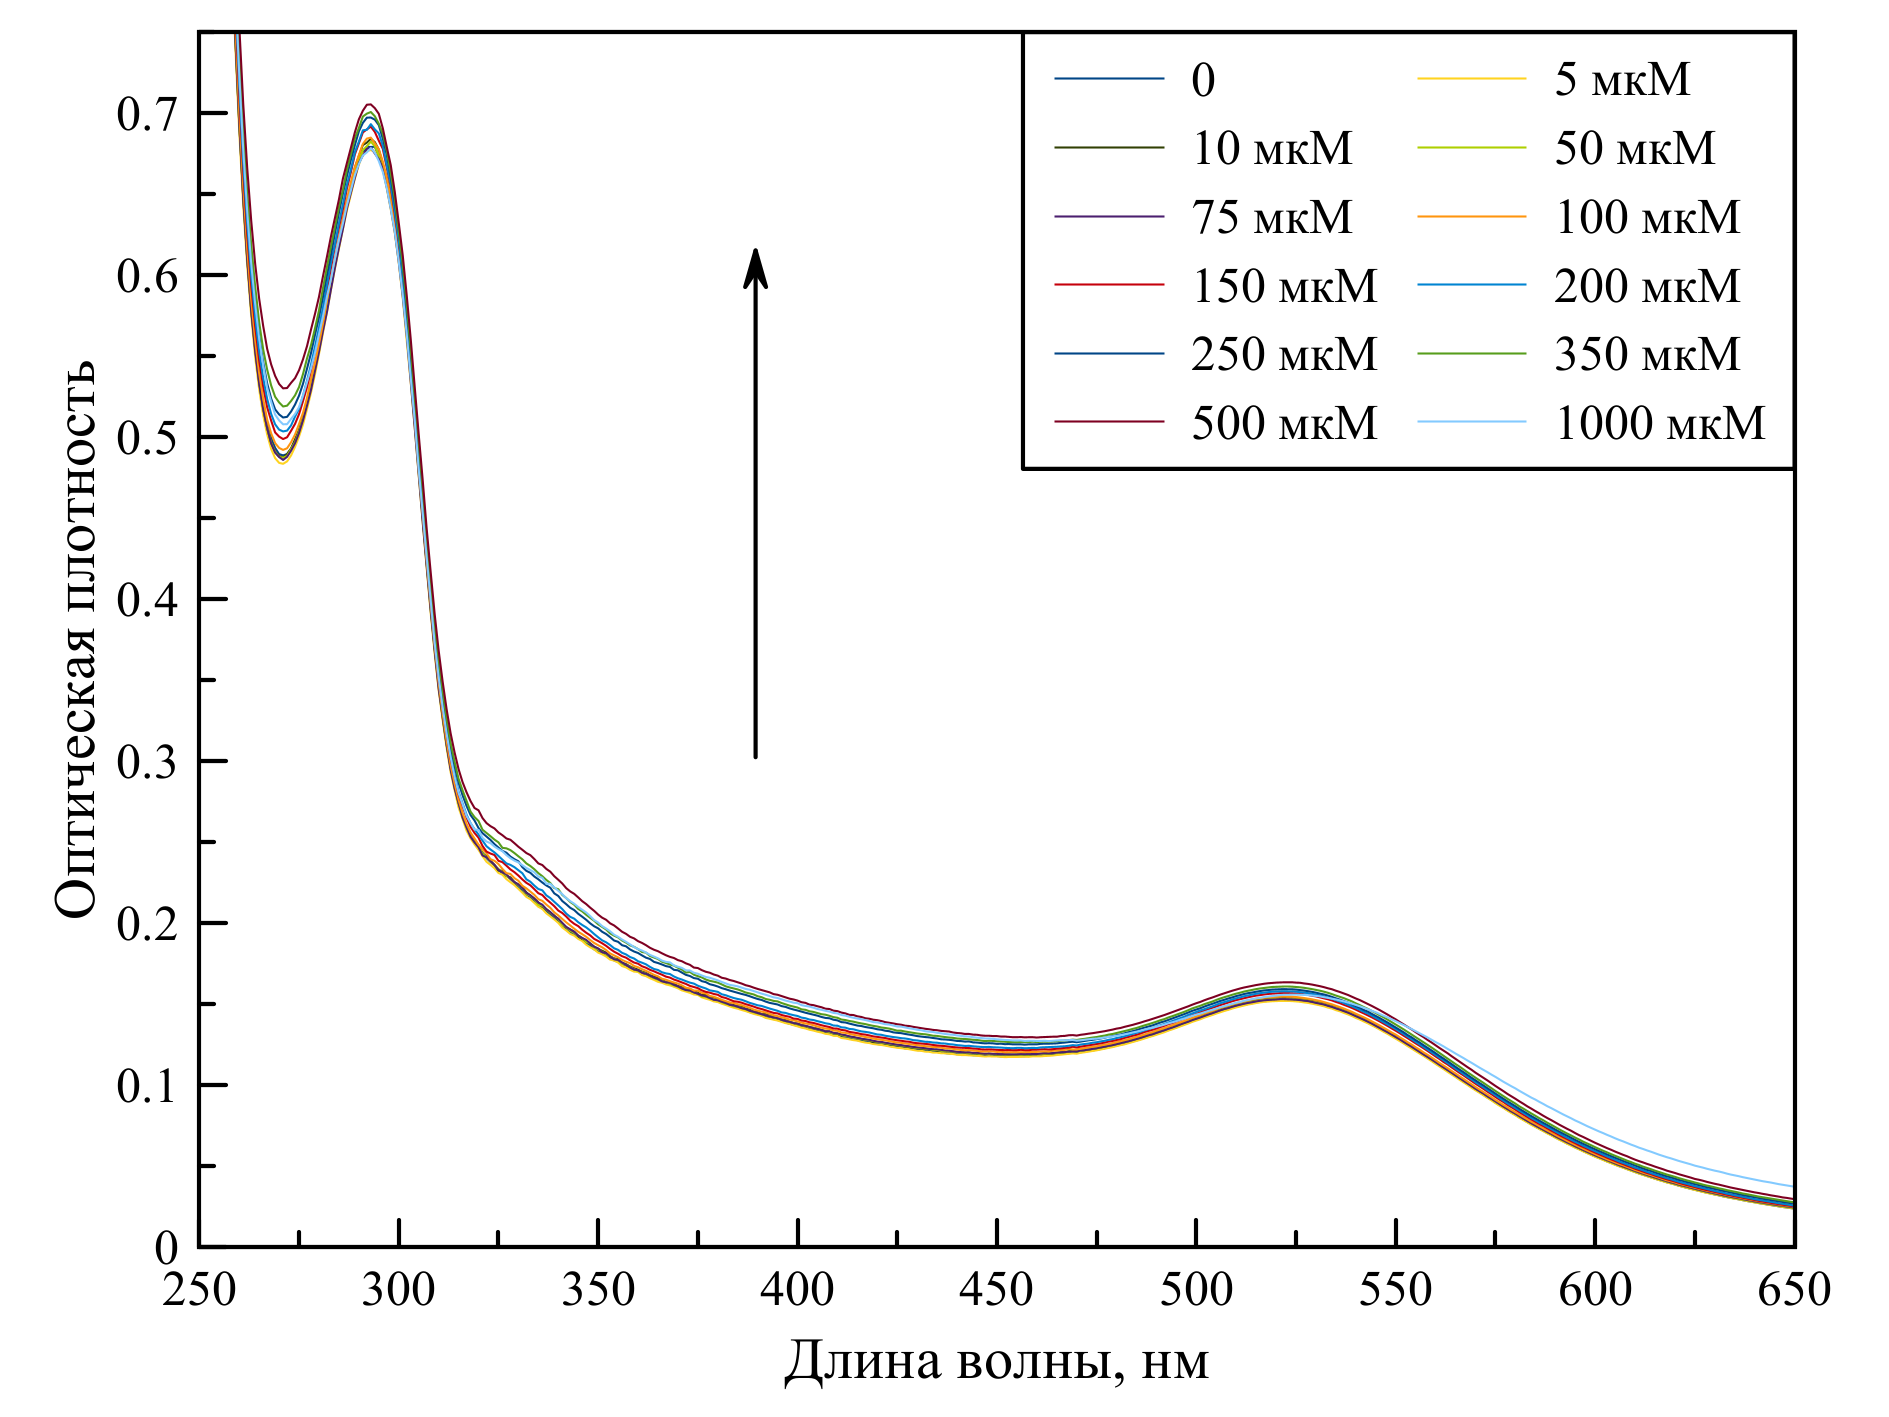
\includegraphics[width=1\linewidth]{attachments/Ni_abs.png}
            \caption{\centering \footnotesize Спектры поглощения золотого нанокластера, стабилизированного тирозином в присутствии ионов никеля.}
        \end{figure}
        \hfill
        \column{0.6\linewidth}
        \begin{figure}
            \centering
            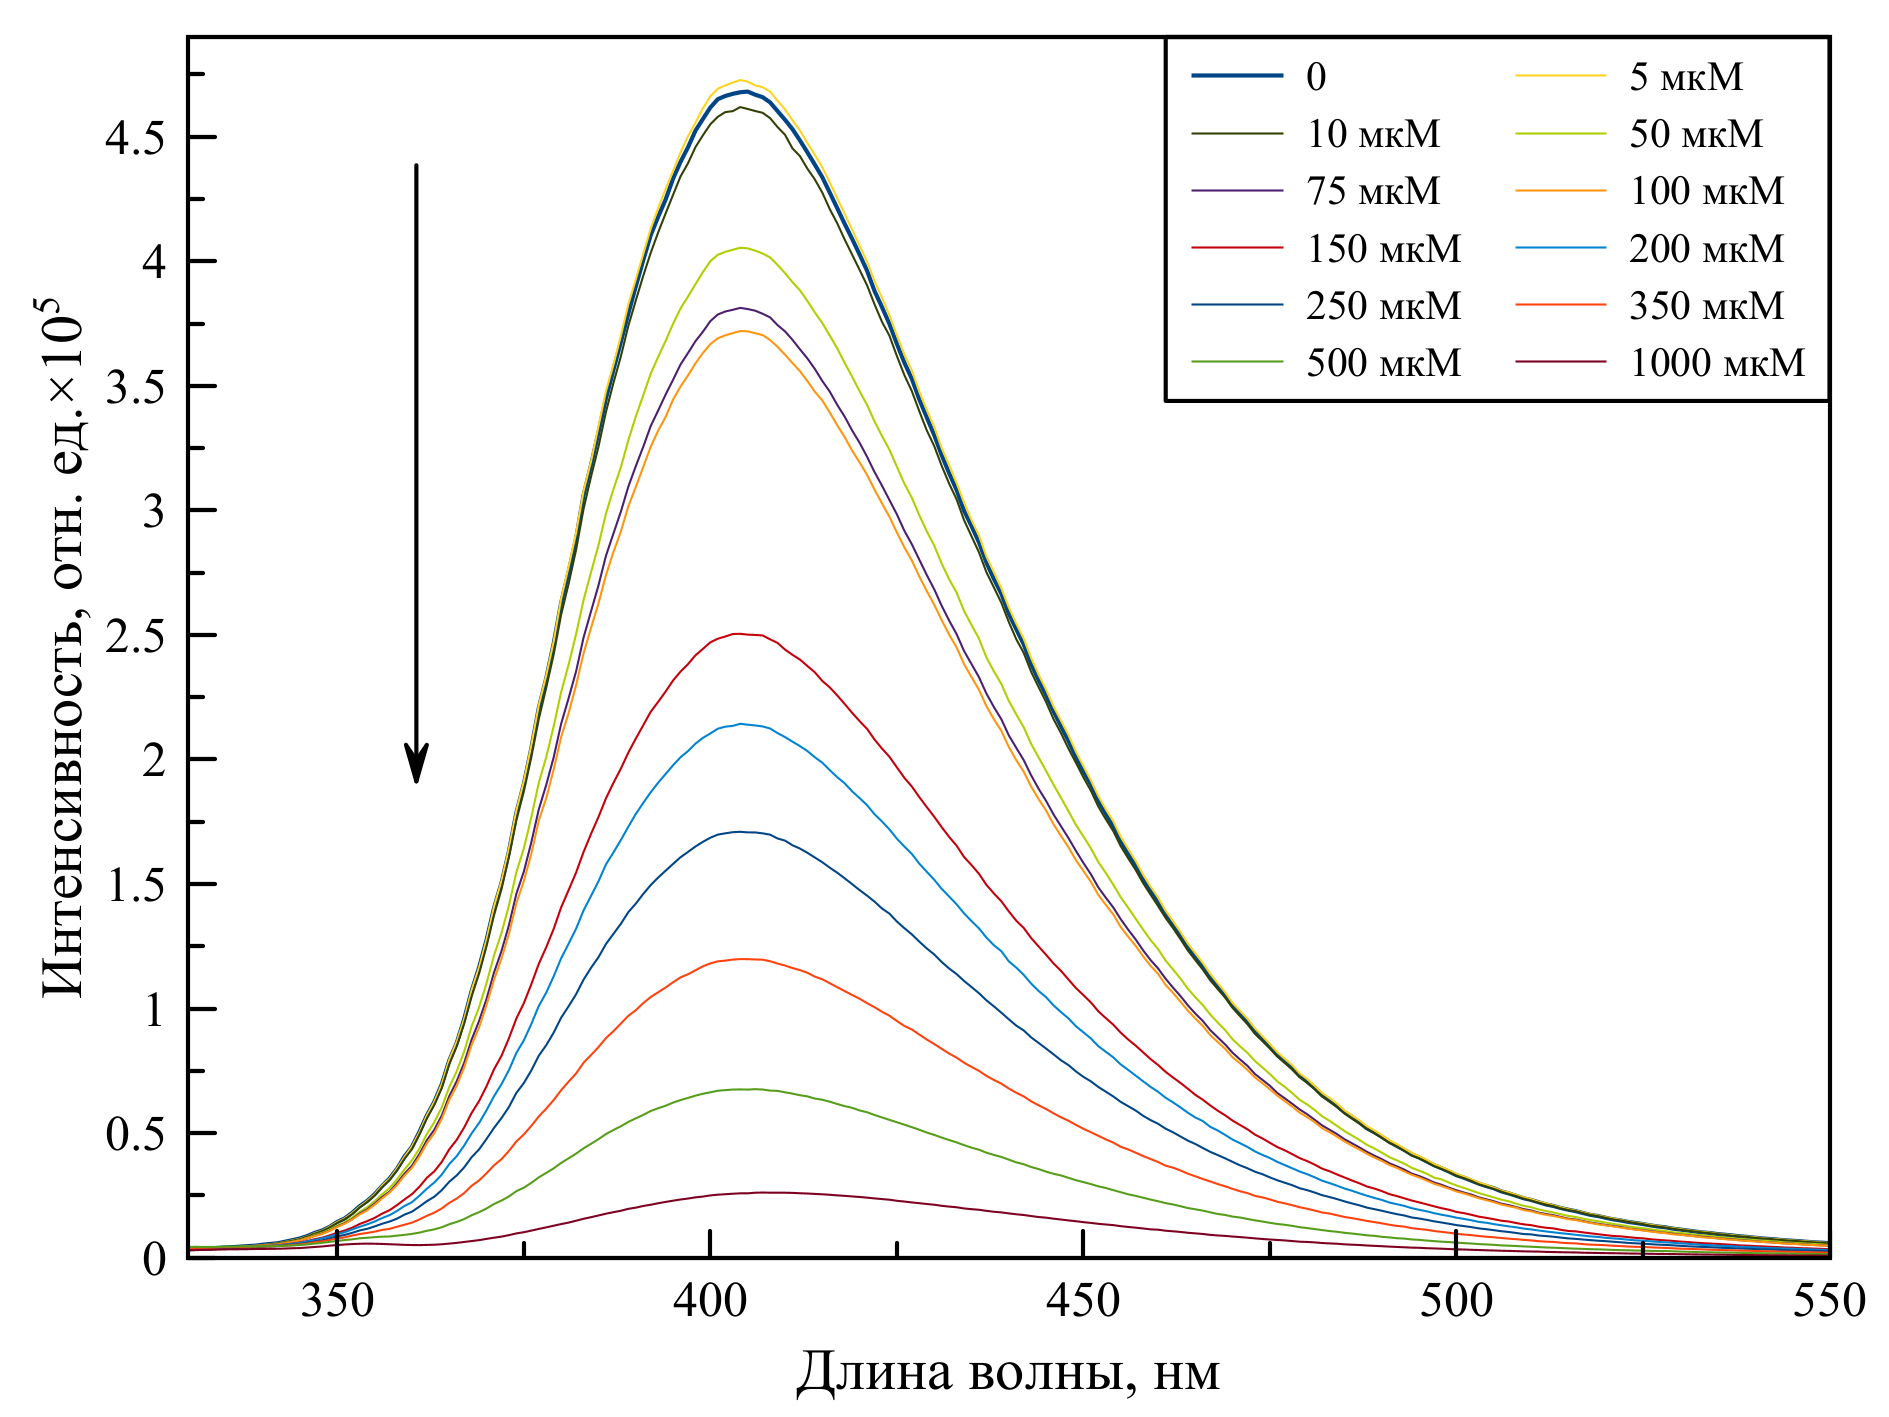
\includegraphics[width=1\linewidth]{attachments/Ni_EM2.png}
            \caption{\centering \footnotesize Корректированные спектры испускания золотого нанокластера, стабилизированного тирозином в присутствии ионов никеля, снятые при длине волны возбуждения равной 315 нм.}
        \end{figure}
    \end{columns}
    \tiny \textcolor{gray}{На рисунках стрелка указывает в направлении увеличения концентрации аналита.}
\end{frame}

\begin{frame}{Взаимодействие с аналитами: никель}
    \centering
    \begin{figure}
        \centering
        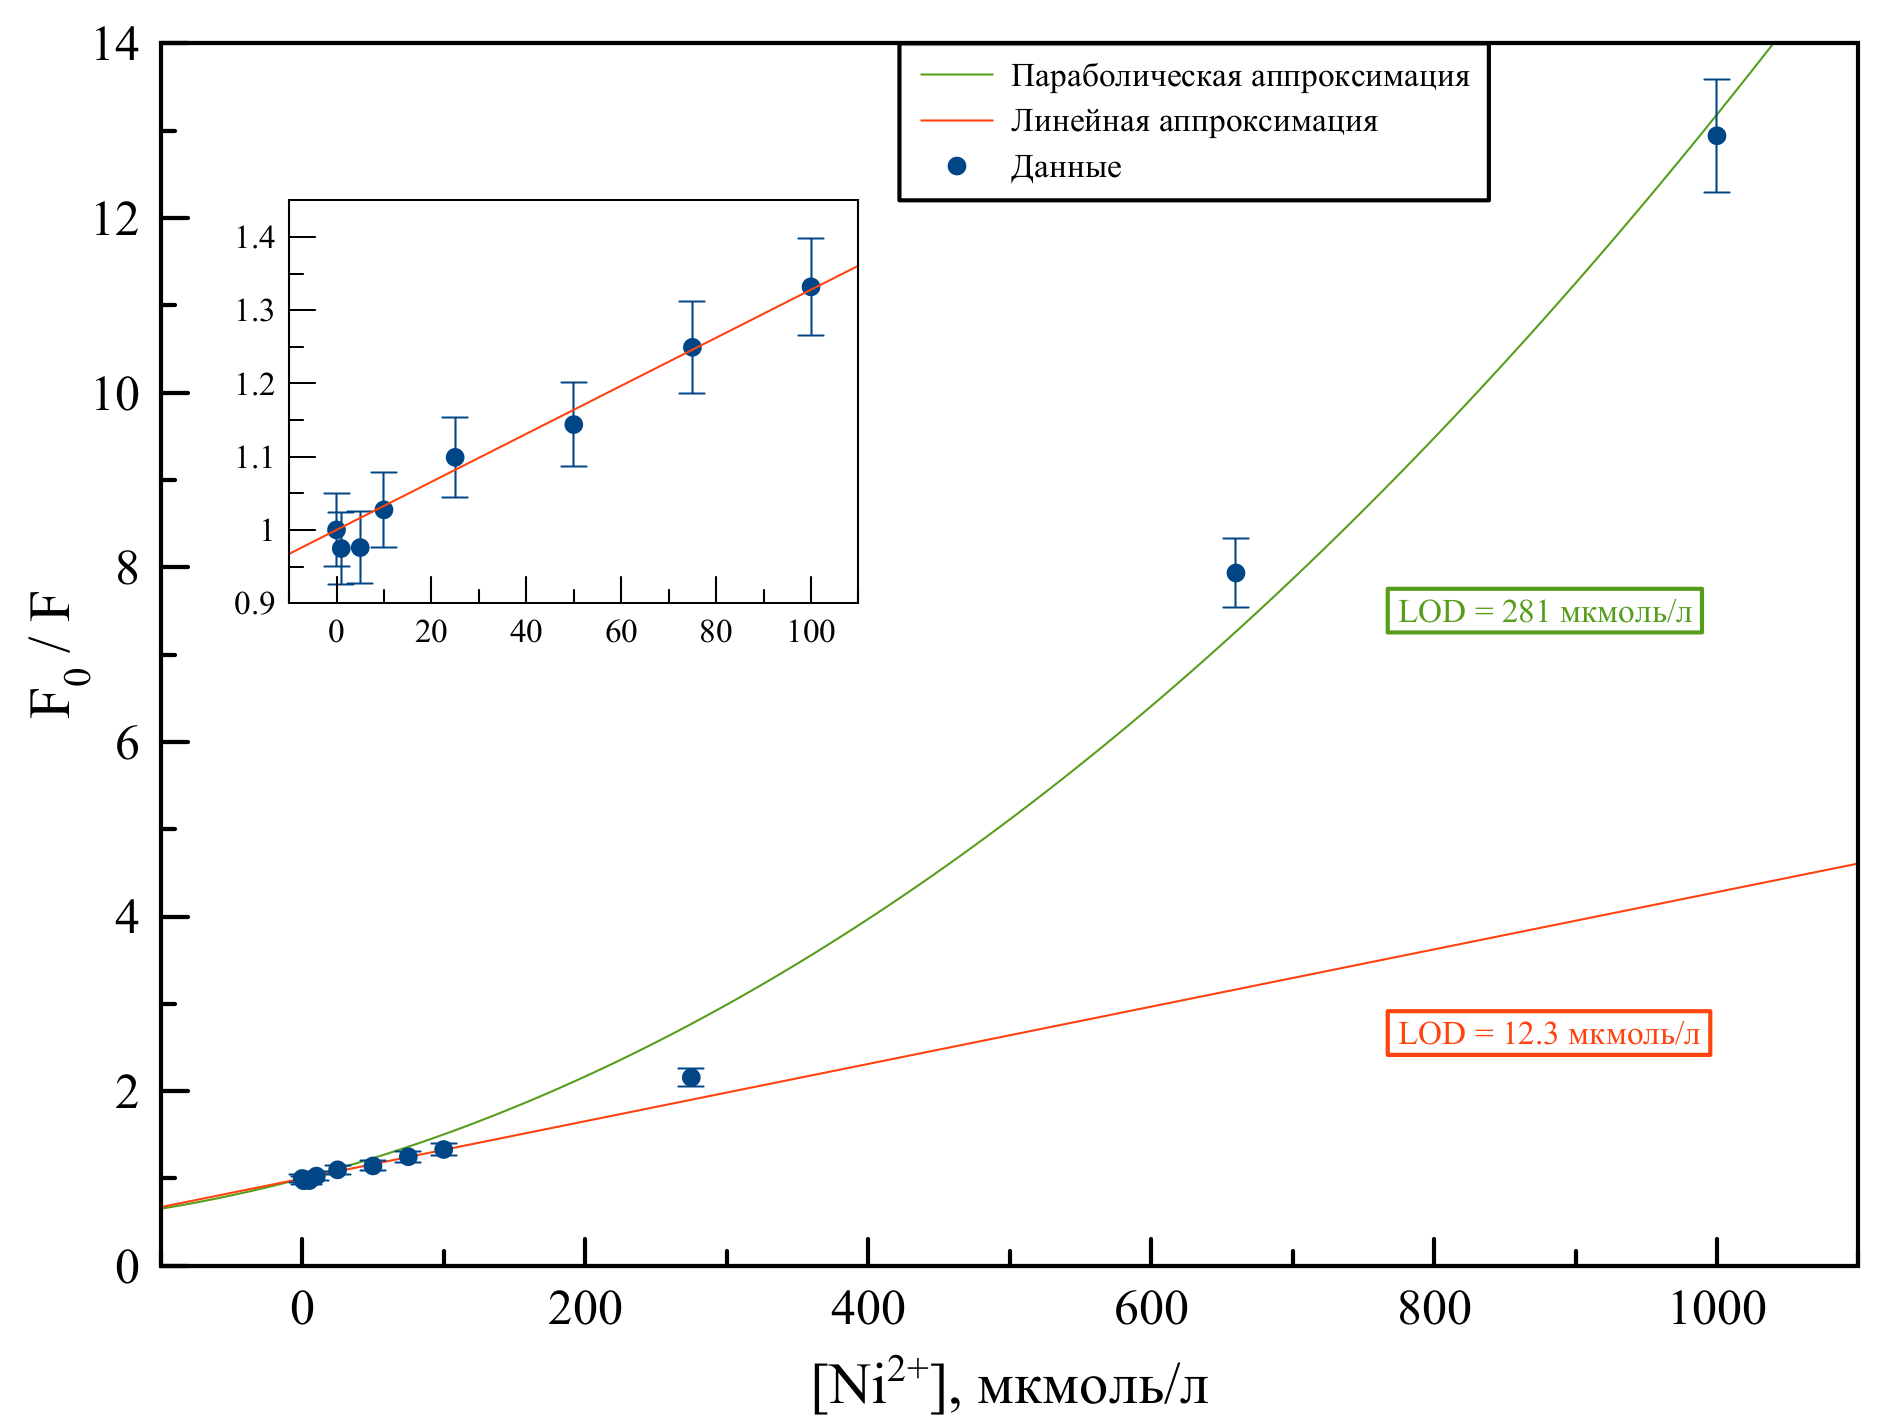
\includegraphics[width=0.8\linewidth]{attachments/Ni_StV_linear100mcM.png}
        \caption{\centering \footnotesize График Штерна-Фольмера для никеля.}
    \end{figure}

\end{frame}

\begin{frame}{Взаимодействие с аналитами: медь}
    \centering
    \begin{columns}[T]
        \column{0.55\linewidth}
        \begin{figure}
            \centering
            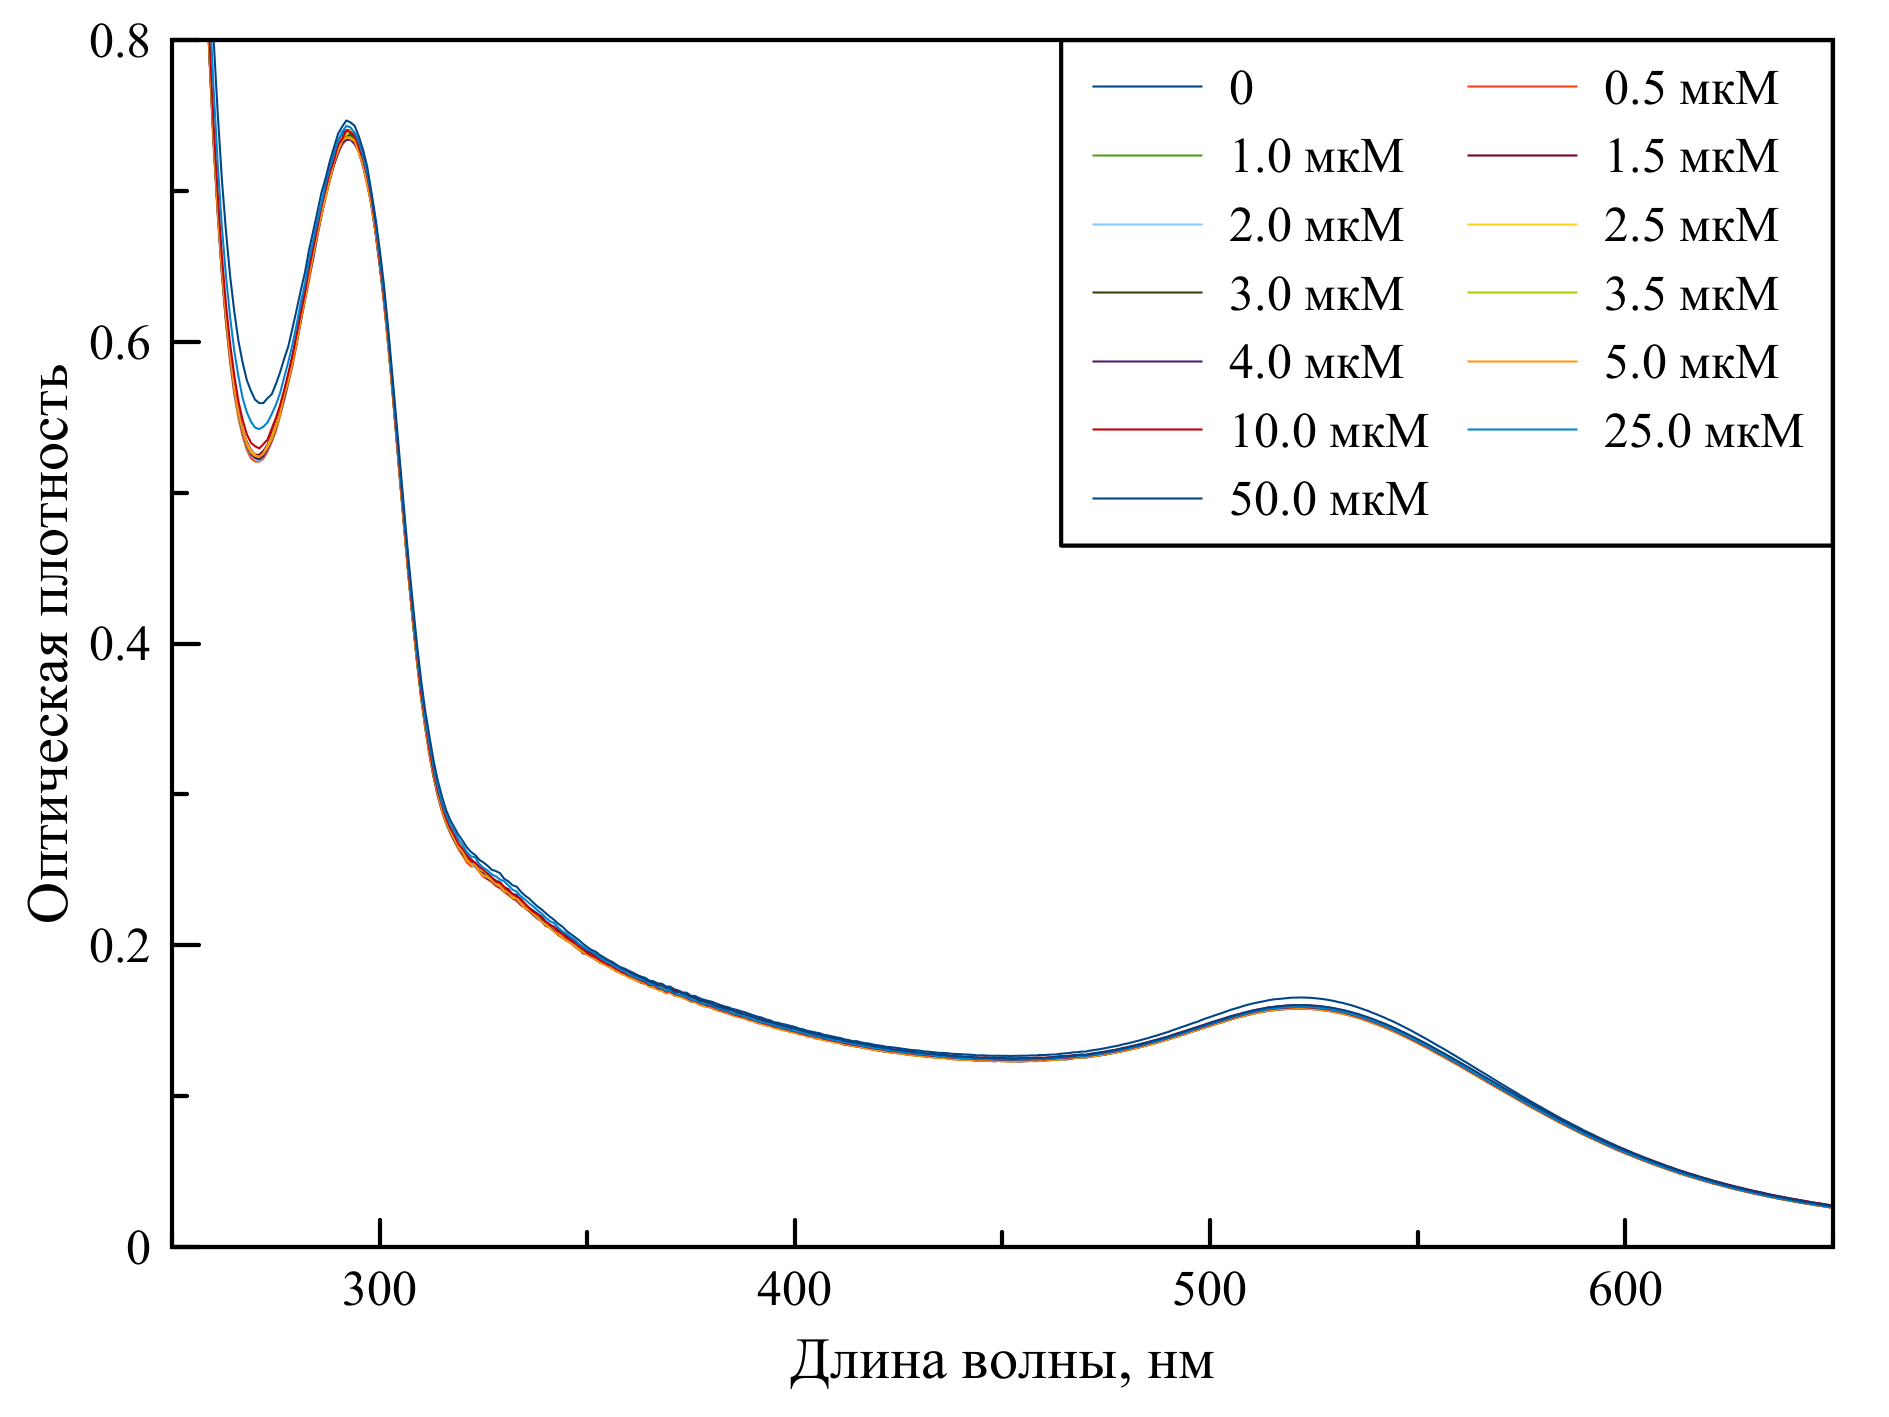
\includegraphics[width=1\linewidth]{attachments/Cu_abs.png}
            \caption{\centering \footnotesize Спектры поглощения золотого нанокластера, стабилизированного тирозином в присутствии ионов меди.}
        \end{figure}
        \hfill
        \column{0.6\linewidth}
        \begin{figure}
            \centering
            
\includegraphics[width=1\linewidth]{attachments/Cu_EM2.png}
            \caption{\centering \footnotesize Корректированные спектры испускания золотого нанокластера, стабилизированного тирозином в присутствии ионов меди, снятые при длине волны возбуждения равной 315 нм.}
        \end{figure}
    \end{columns}
    \tiny \textcolor{gray}{На рисунках стрелка указывает в направлении увеличения концентрации аналита.}
\end{frame}

\begin{frame}{Взаимодействие с аналитами: медь}
    \centering
    \begin{figure}
        \centering
        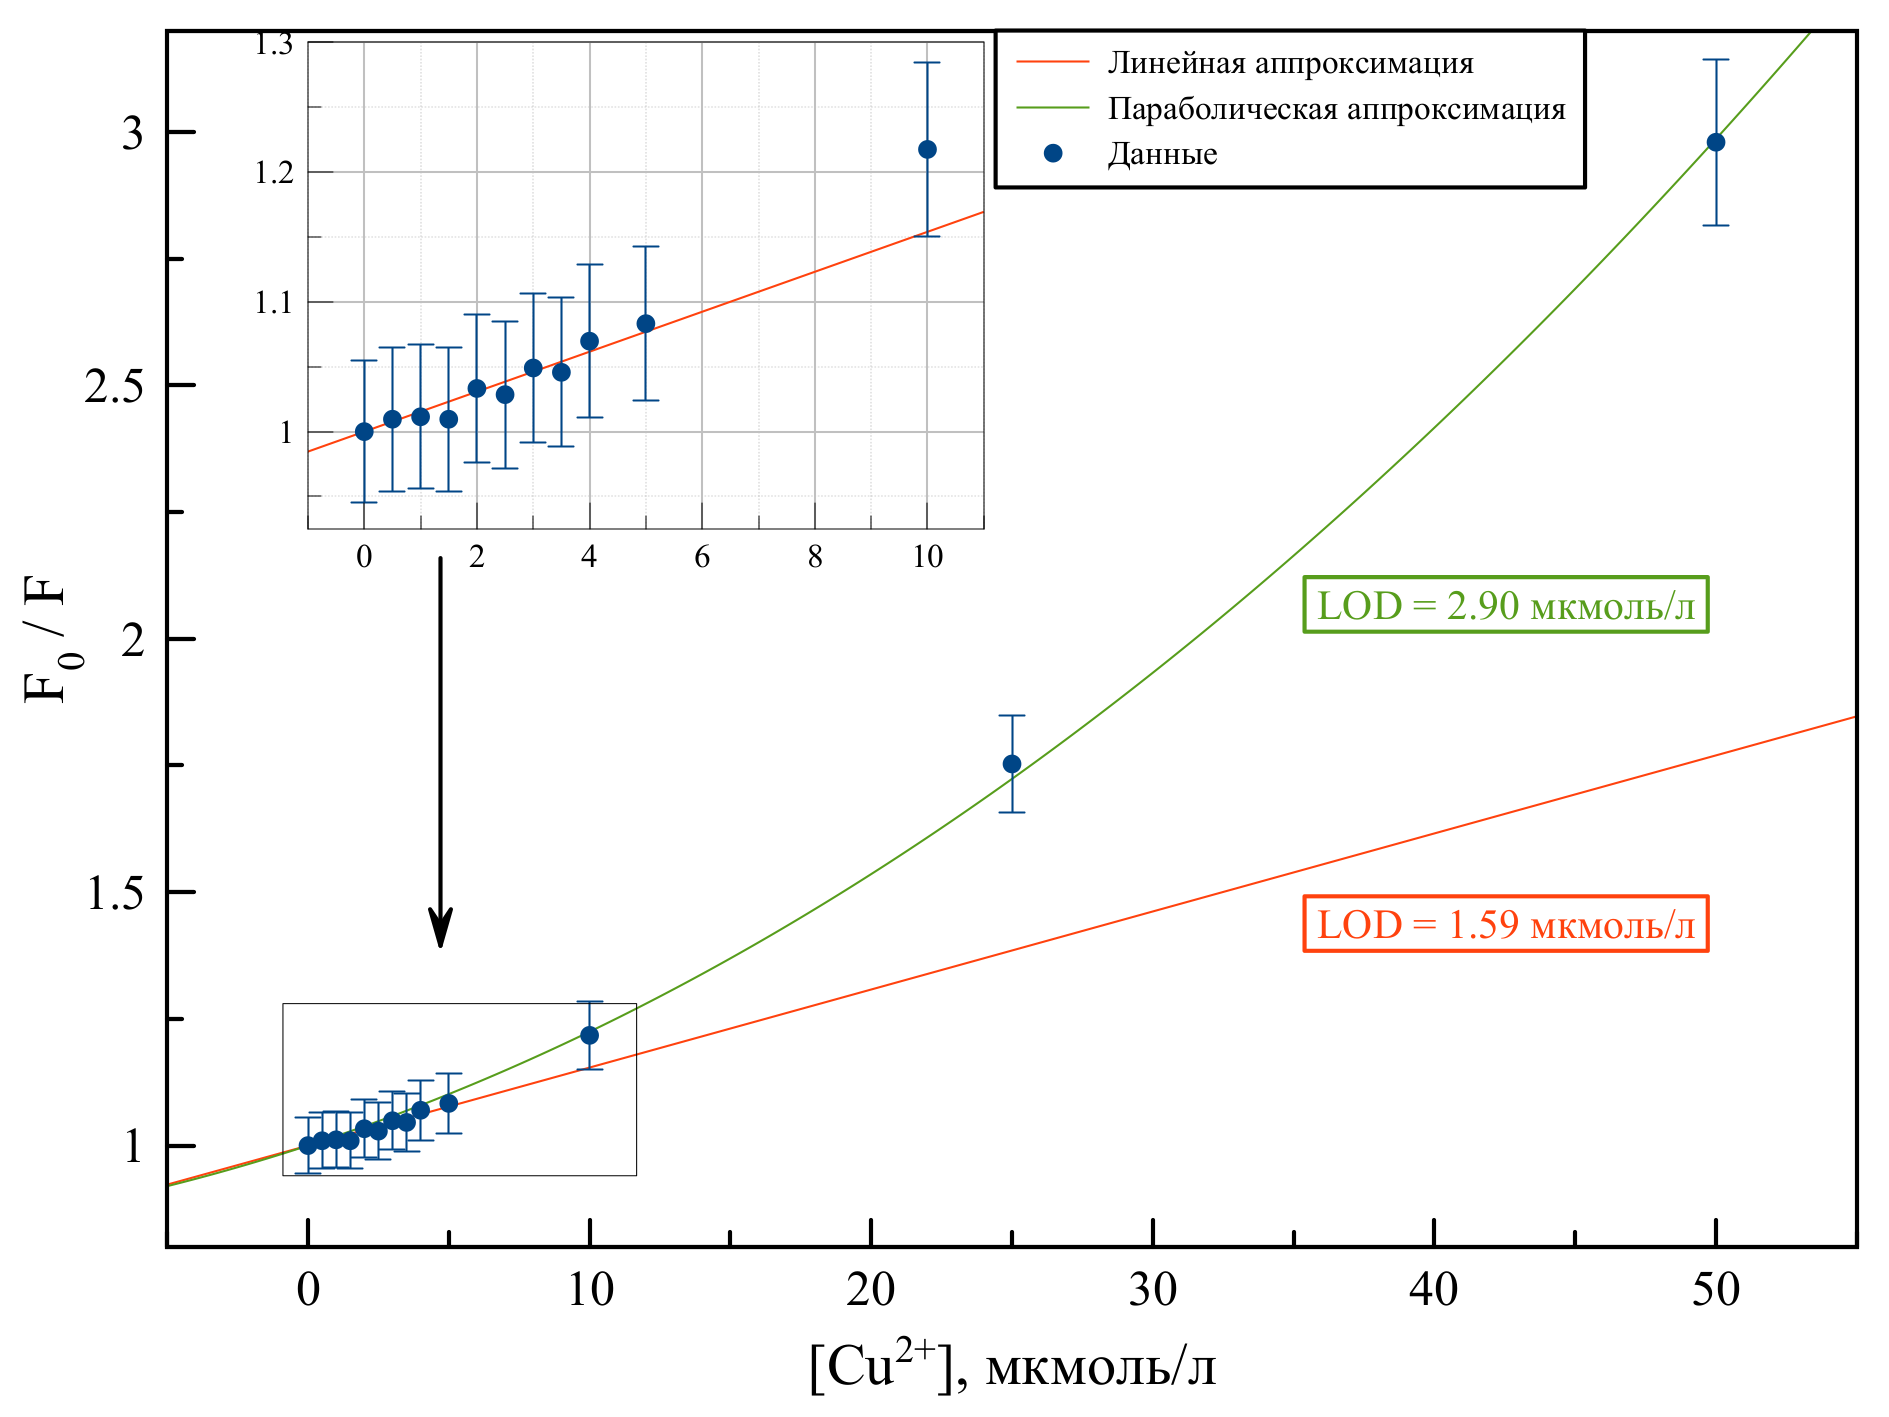
\includegraphics[width=0.8\linewidth]{attachments/Cu_StV.png}
        \caption{\centering \footnotesize График Штерна-Фольмера для меди.}
    \end{figure}

\end{frame}

\begin{frame}{Сравнение сенсорных свойств}
    \begin{table}[H]
	\centering
	\caption{Сравнение предела обнаружения и предельно допустимых концентраций для представленных аналитов}
	\label{tab:LOD-TVL}
	\begin{tabular}{|c|c|c|}
	\hline
	\textbf{Аналит}                & \textbf{Медь}         & \textbf{Никель}  \\\hline\hline
	Предел обнаружения, $\text{мкмоль}/\text{л}$   & \textcolor{green}{1.59} & \textcolor{red}{12.3} \\\hline
	ПДК\footnote{\scriptsize Предельно допустимая концентрация. \\ Источник: САНПИН 1.2.3685-21. Санитарные правила и нормы по обеспечению безопасности при производстве, хранении и перевозке продукции, подлежащей обязательному техническому регулированию. — Москва, 2021 ; — Приказ Минздрава России от 30.12.2020 № 1036н.},
    $\text{мкмоль}/\text{л}$   &    15.7                 &   3.4                \\\hline
	Линейный диапазон, до & $10~\text{мкмоль}/\text{л}$ & $100~\text{мкмоль}/\text{л}$\\\hline\hline
    Время жизни люминесценции & $4.27~\text{нс}$ & $5.07~\text{нс}$\\\hline
	\end{tabular}
	\end{table}



\end{frame}

\begin{frame}{Взаимодействие лиофилизованного кластера: медь}
    \centering
    \begin{columns}[T]
        \column{0.55\linewidth}
        \begin{figure}
            \centering
            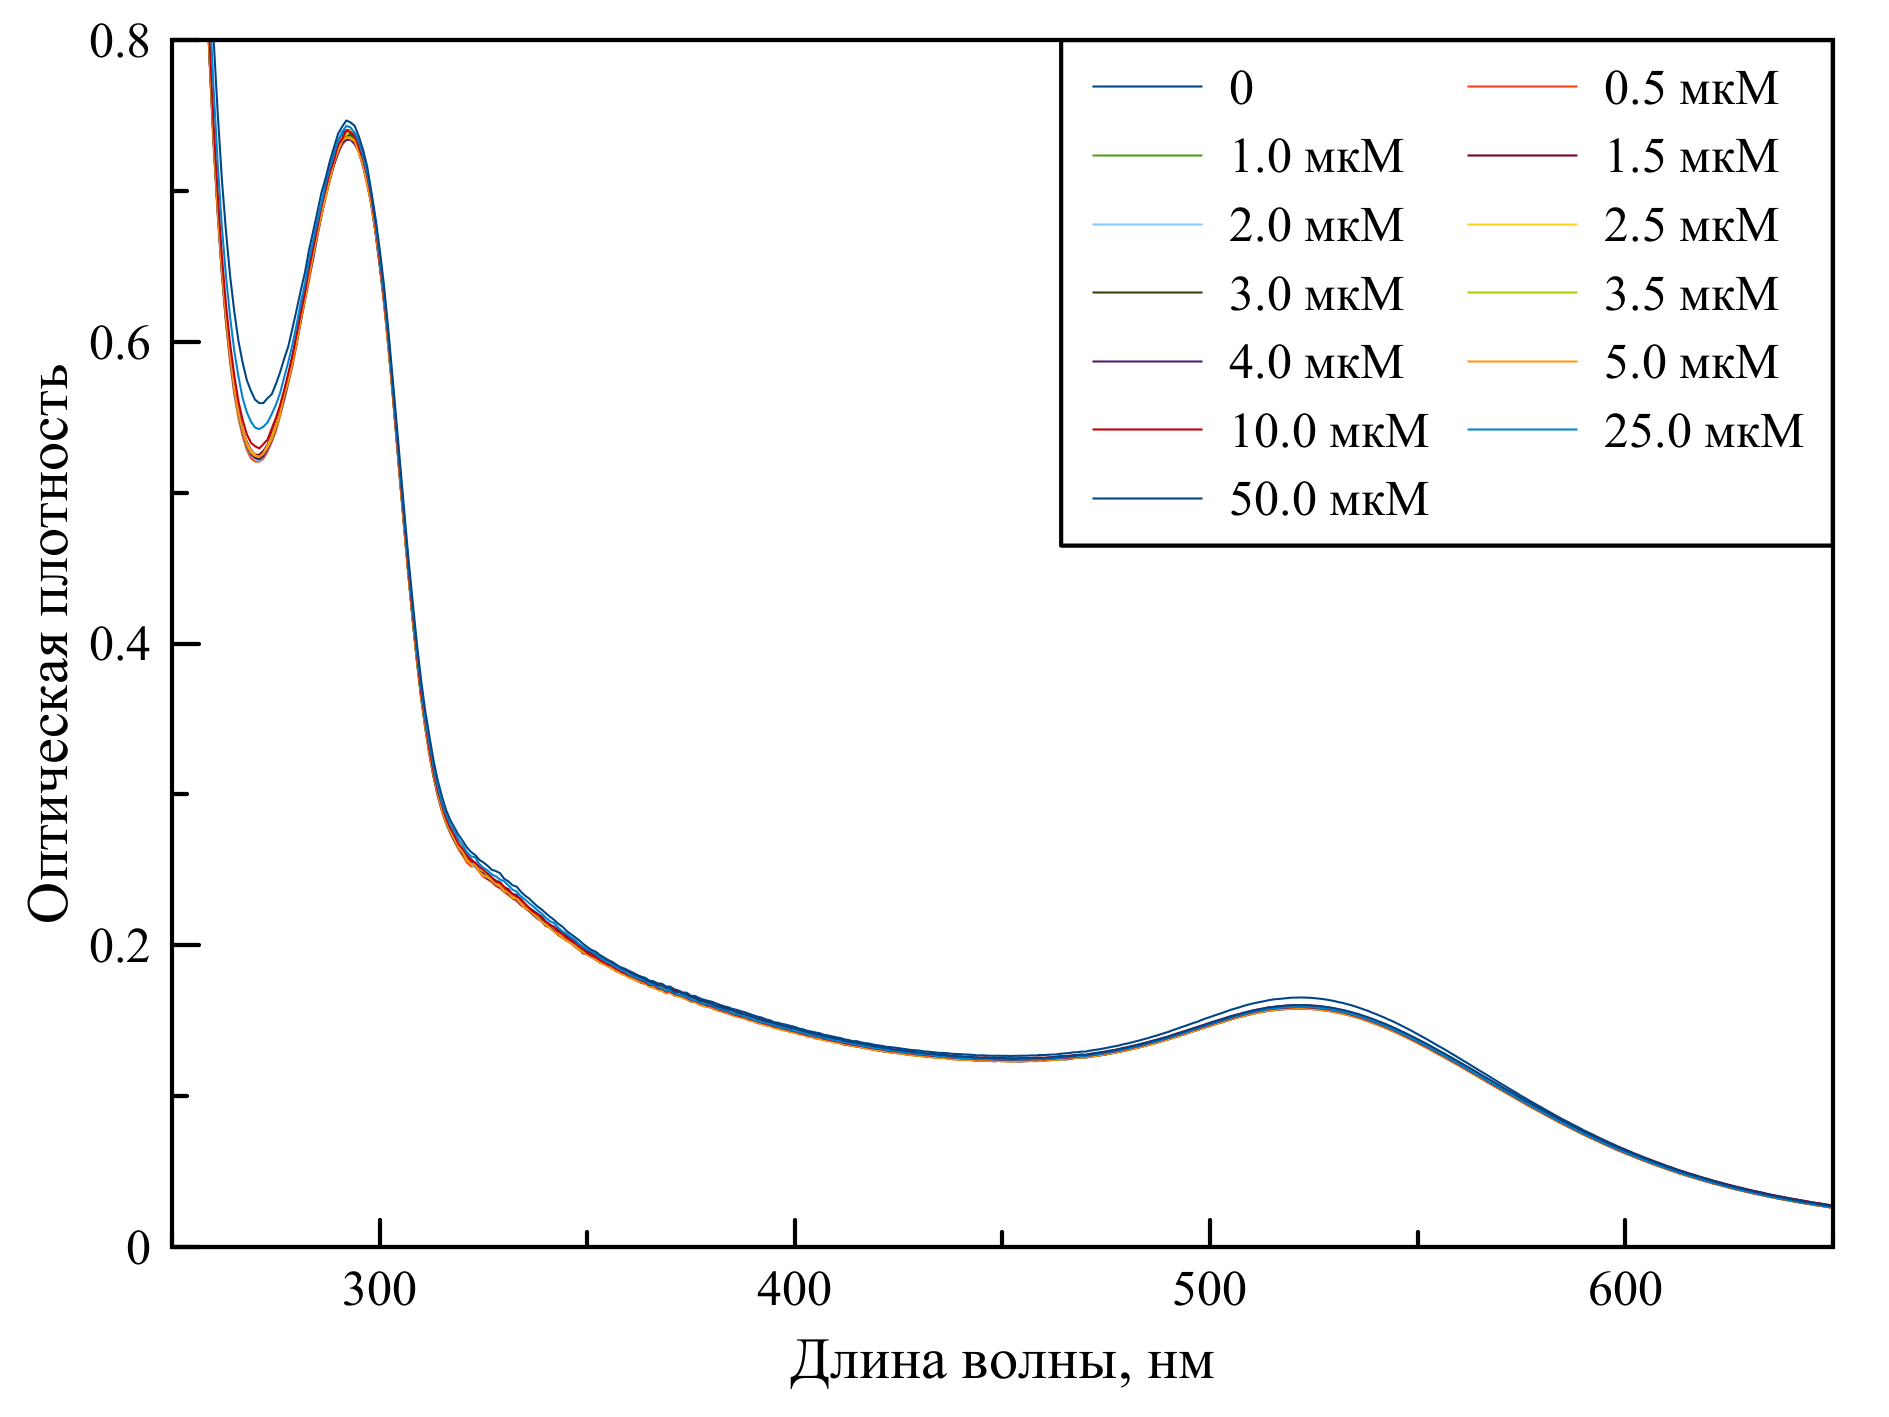
\includegraphics[width=1\linewidth]{attachments/Cu_abs.png}
            \caption{\centering \footnotesize Спектры поглощения для перерастворённого кластера в присутствии ионов меди.}
        \end{figure}
        \hfill
        \column{0.6\linewidth}
        \begin{figure}
            \centering
            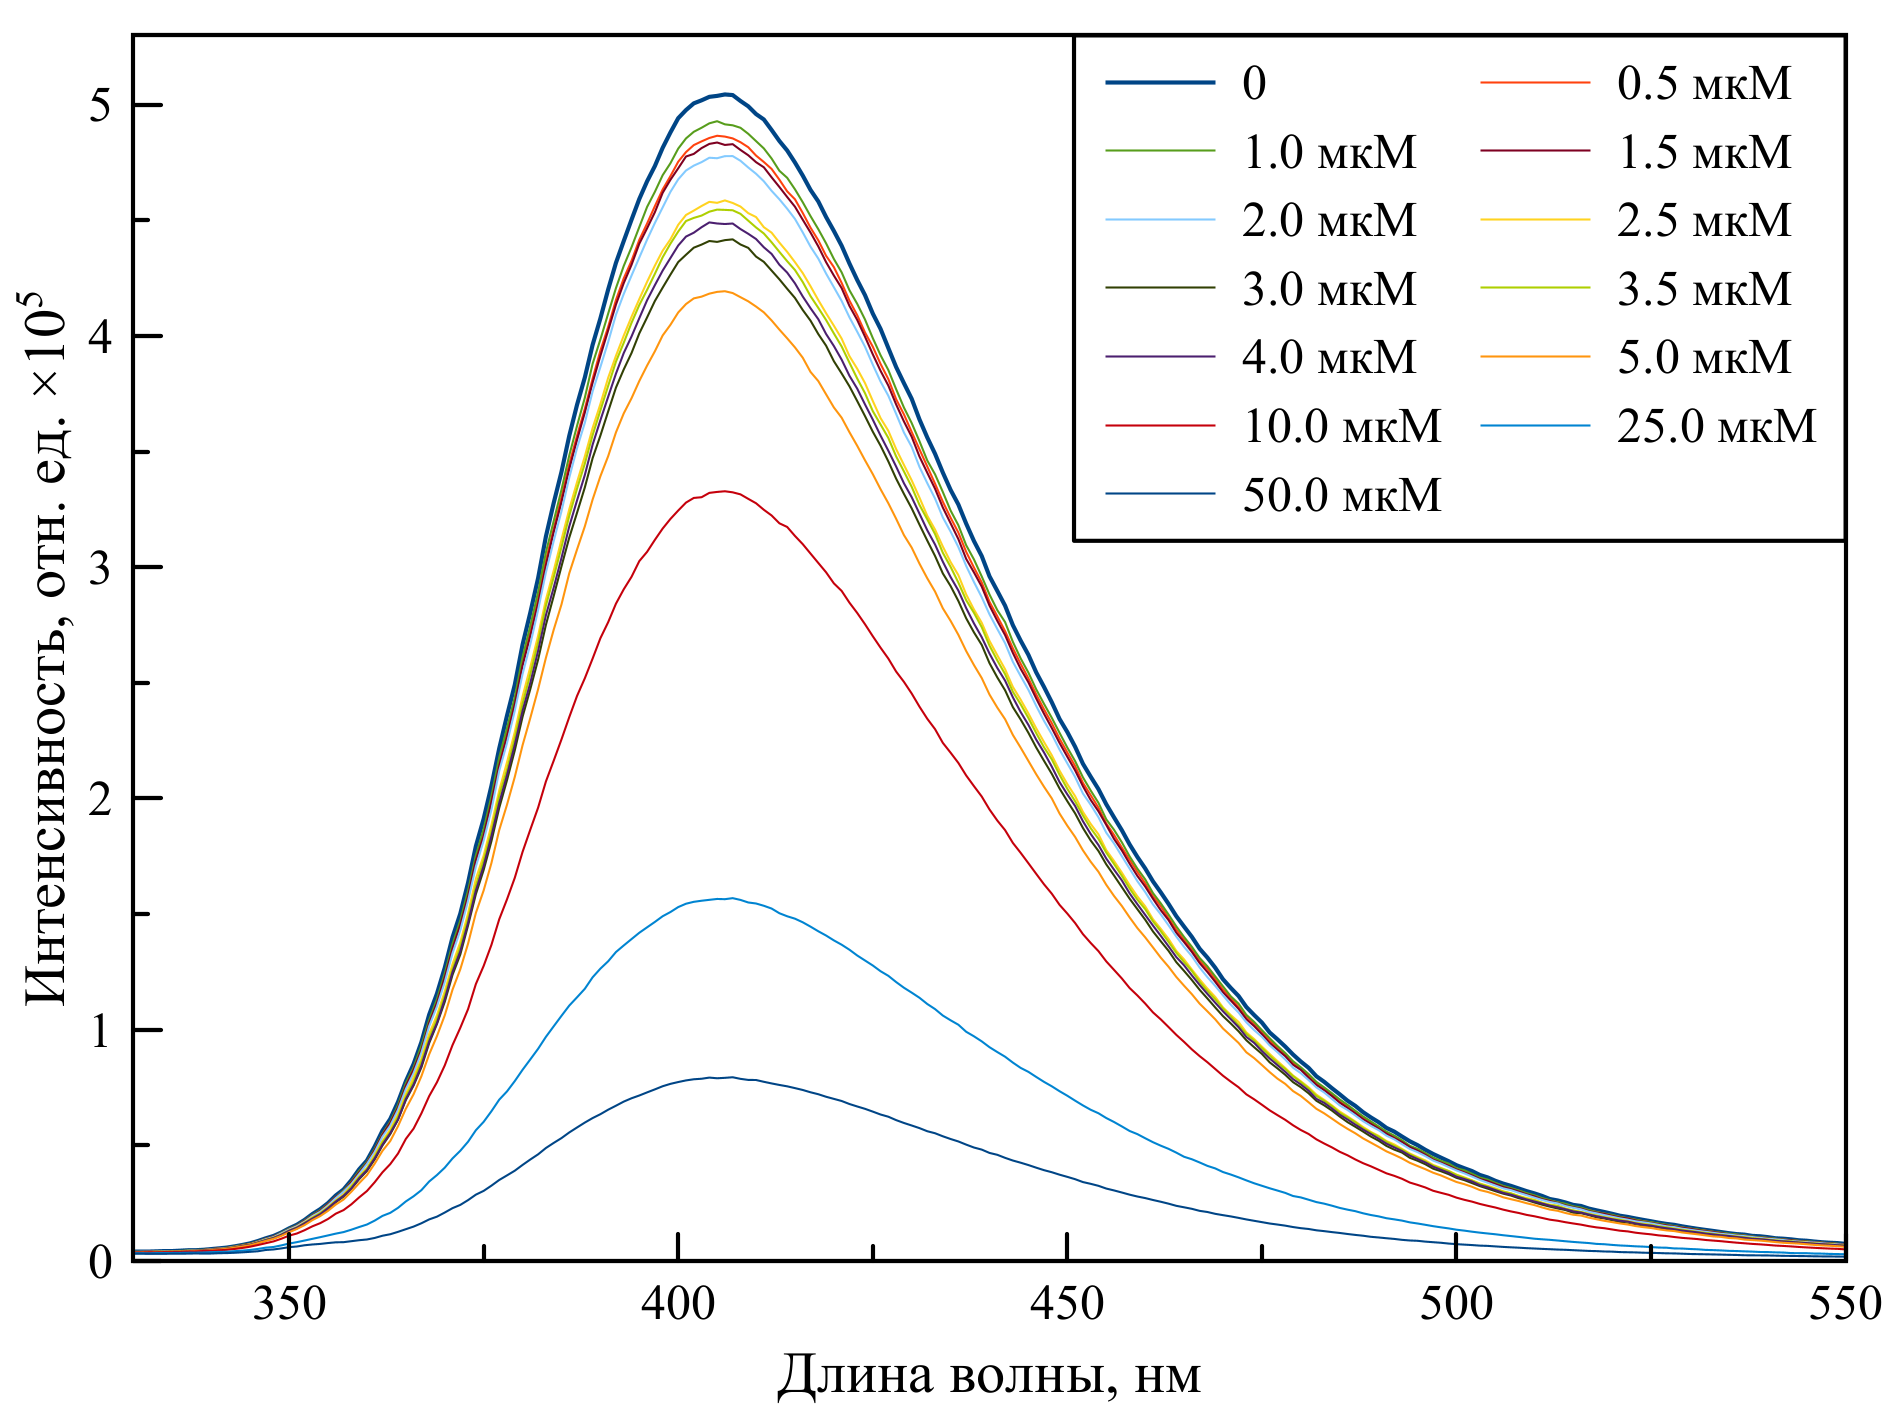
\includegraphics[width=1\linewidth]{attachments/Luoph_Cu_EM2.png}
            \caption{\centering \footnotesize Корректированные спектры испускания перерастворённого кластера в присутствии ионов меди, снятые при длине волны возбуждения равной 315 нм.}
        \end{figure}
    \end{columns}
\end{frame}

\begin{frame}{Взаимодействие лиофилизованного кластера: медь}
    \centering
    \begin{figure}
        \centering
        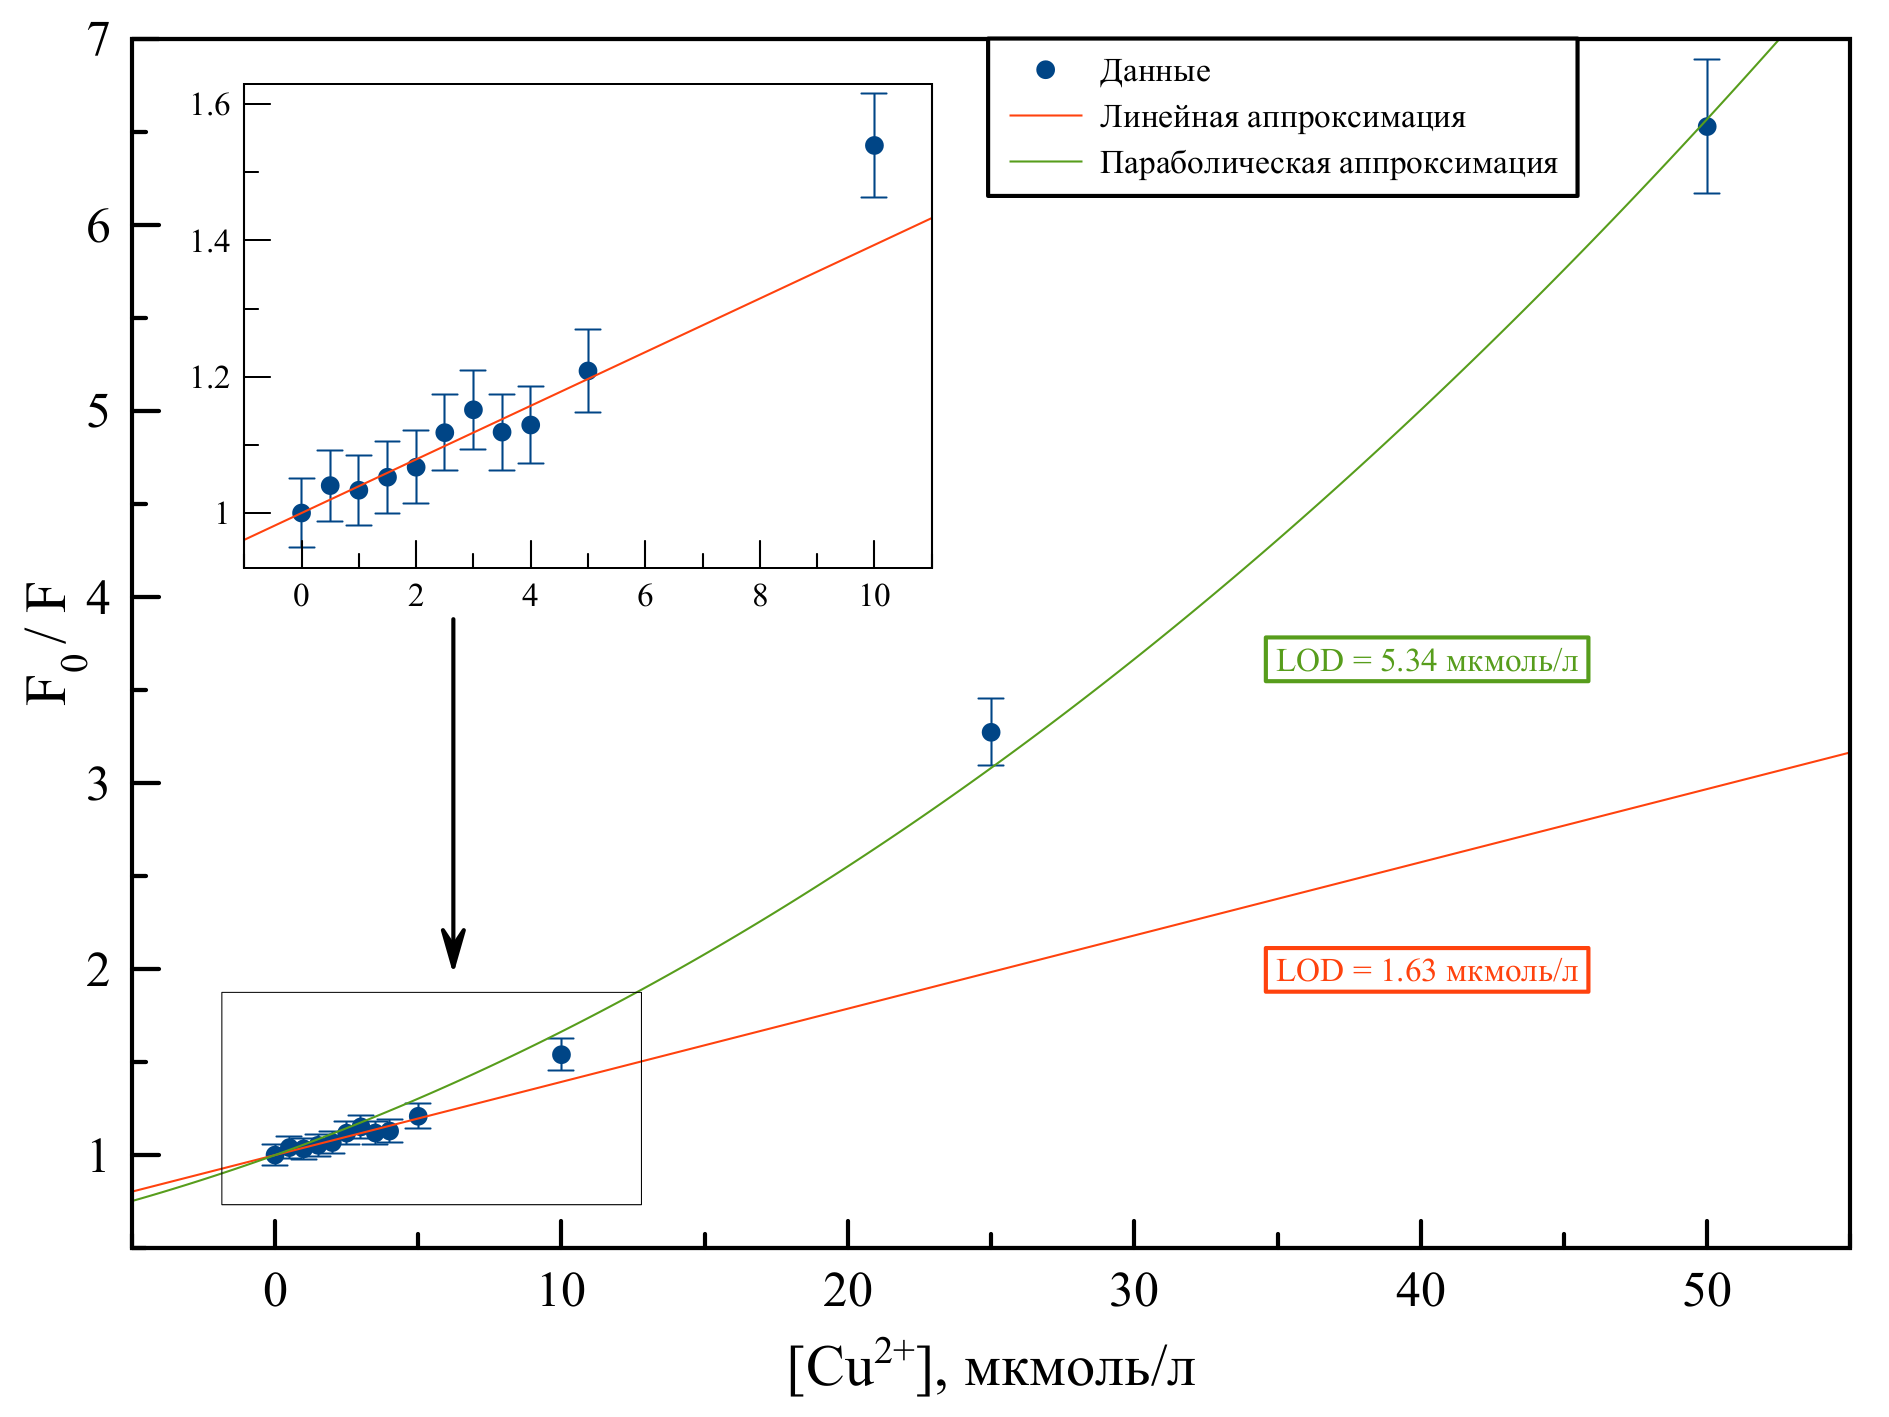
\includegraphics[width=0.8\linewidth]{attachments/Luoph_Cu_StV.png}
        \caption{\centering \footnotesize График Штерна-Фольмера для перерастворённого кластера в присутствии ионов меди.}
    \end{figure}

\end{frame}

\begin{frame}{Слепой тест}
    \begin{table}[h!]
	\centering
	\caption{Результаты определения ионов $\text{Cu}^{2+}$ в слепых пробах методом Штерна-Фольмера.}
	\label{tab:blind_test_results}
	\begin{tabular}{|c|c|c|c|c|}
	\hline
	№ образца & Введено $\text{Cu}^{2+}$, мкМ & Найдено $\text{Cu}^{2+}$, мкМ & Recovery, \%  \\ \hline\hline
	        1 & $0.85$             & $0.94  \pm 0.05$             & 110.6    \\ \hline
	        2 & $2.50$             & $2.40  \pm 0.11$             & 96.0     \\ \hline
	        3 & $4.70$             & $4.80  \pm 0.25$             & 102.1    \\ \hline
	        4 & $6.40$             & $6.50  \pm 0.31$             & 101.6    \\ \hline
	        5 & $8.20$             & $8.00  \pm 0.39$             & 97.6     \\ \hline
            6 & $12.60$            & $10.80 \pm 0.60$             & 85.7     \\ \hline
	\end{tabular}
	\end{table}
\end{frame}

\begin{frame}{Результаты}
    \centering
    \begin{enumerate}
        \item Получен и охарактеризован золотой нанокластер, стабилизированный тирозином.
        \vfill
        \item Полученная система обладает чувствительностью к ионам меди и никеля. \emph{Система позволяет детектировать ионы меди ниже предела допустимой концентрации}.
        \vfill
        \item Регидратированный лиофилизат сохраняет исходные фотофизические свойства $\to$ возможно использование системы в качестве готового аналитического набора.
    \end{enumerate}
\end{frame}

\end{document}